% DAVID AND ANMOL: IMPORTANT THING TO ADD.  DAVID'S REFINEMENT OF LOCAL VERSUS GLOBAL OF STEADY STATES.  PUT THIS IN AS A REFINEMENT OF THE ``PHILLIPON'' INTUITION SECTION AND
% LINK TO ALBENESI AND ARMENTER.


\documentclass[12pt]{article}


\usepackage{amsmath,amssymb,amsthm,enumerate,graphicx}
\usepackage{ifthen,latexsym,syntonly}
\usepackage{setspace}
%\usepackage[showrefs]{refcheck}  %use this to show equation and section labels
\usepackage[round,comma,authoryear]{natbib}   % for natbib
\usepackage{subfigure}
\usepackage{float}
\usepackage{epstopdf}
\usepackage{hyperref}
\usepackage{bm}
\usepackage{soul}
\usepackage{graphicx}

%commands to allow for easy editing
\usepackage[usenames,dvipsnames]{color}

%command to insert editing comments or track changes
\newcommand{\dge}[1]{\textcolor{blue}{$^{\textrm{dge}}${#1}}}
\newcommand{\apb}[1]{\textcolor{magenta}{$^{\textrm{apb}}${#1}}}
\newcommand{\tjs}[1]{\textcolor{red}{$^{\textrm{tjs}}${#1}}}

\bibliographystyle{mynat}


\onehalfspacing


   % for natbib
%\bibpunct{(}{)}{,}{a}{}{,}  % for natbib
%                            % need to have mynat.bst in an accesssible directory


\bibpunct{(}{)}{,}{a}{}{,}  % for natbib
                            % need to have mynat.bst in an accesssible directory

\newcommand{\EE}{\mathbb E}
\newtheorem{theorem}{Theorem}[section]
\newtheorem{remark}[theorem]{Remark}
\newtheorem{assumption}[theorem]{Assumption}
%\newtheorem{case}[theorem]{Case}
\newtheorem{claim}[theorem]{Claim}
%\newtheorem{conclusion}[theorem]{Conclusion}
\newtheorem{corollary}[theorem]{Corollary}
\newtheorem{condition}[theorem]{Condition}
\newtheorem{criterion}[theorem]{Criterion}
\newtheorem{definition}[theorem]{Definition}
\newtheorem{example}[theorem]{Example}
\newtheorem{lemma}[theorem]{Lemma}
\newtheorem*{lemma*}{Lemma}
\newtheorem{problem}[theorem]{Problem}
\newtheorem{proposition}[theorem]{Proposition}
\newtheorem*{proposition*}{Proposition}
%\newtheorem{solution}[theorem]{Solution}
%\newtheorem{summary}[theorem]{Summary}
\newtheorem{thm}[theorem]{Theorem}
\newcommand{\var}{\text{var}}
\newcommand{\cov}{\text{cov}}
\newcommand{\barB}{{\overline B}}
\newcommand{\barC}{{\overline C}}
\newcommand{\pbar}{{\overline p}}
\newcommand{\bbar}{{\overline b}}
\newcommand{\mubar}{{\overline \mu}}


\setlength{\oddsidemargin}{.05in} \setlength{\topmargin}{-.45in}
\setlength{\textwidth}{6.4in} \setlength{\textheight}{8.5in}


%\pagestyle{empty}

\title {Optimal Taxation with Incomplete Markets}
%\author{Anmol Bhandari, David Evans, Mikhail Golosov, Thomas J. Sargent}
\author{\textbf{Anmol Bhandari}\\apb296@nyu.edu \and \textbf{David Evans} \\ \texttt{dgevans@nyu.edu} \and \textbf{Mikhail Golosov}\\\texttt{golosov@princeton.edu} \and \textbf{Thomas J. Sargent} \\ \texttt{thomas.sargent@nyu.edu}
}

\begin{document}

\maketitle



\begin{abstract}  This paper characterizes tax and debt dynamics in Ramsey plans for incomplete markets economies that generalize
an \citet{Aiyagari2002} economy by allowing a single asset traded by the government  to be risky.
Long run debt and tax dynamics can be attracted  not only to the first-best continuation allocations discovered by \citeauthor{Aiyagari2002} for quasi-linear preferences, but instead
 to a continuation allocation  associated with a level of (marginal-utility-scaled) government debt that would prevail in a Lucas-Stokey
economy that starts from a particular initial level of government debt.  The paper formulates, analyzes, and numerically solves  Bellman equations
for two value functions for a Ramsey planner, one for $t \geq 1$, the other for $t=0$.



\end{abstract}


\noindent\textsc{Keywords:} Complete markets, incomplete markets, Ramsey plan, taxes, debt, competitive equilibrium, implementability constraints,
dynamic programming squared

\newpage

\section{Introduction}


\begin{quote}
``$\ldots$ the option to issue state-contingent debt is important: tax policies that
are optimal under uncertainty have an essential `insurance' aspect to them.'' \quad \citet[p.~88]{LucasJr.1983}
\end{quote}



Controversies sparked by  \citet{Reinhart2010} motivate us to reassess what we know and don't know about two elementary questions.
How much government debt is optimal? And  is government debt  even a pertinent state variable? % in a recursive formulation of a Ramsey problem?
\citet{LucasJr.1983} and \citet{Aiyagari2002} offer  different answers to these two
questions in the context of  economic environments that are identical in all respects but one: \citet{LucasJr.1983} let the government to issue
a complete set of Arrow securities, while   \citet{Aiyagari2002} restrict the government to issue only a one-period risk-free government bond.  For
\citeauthor{LucasJr.1983}, under an optimal tax and debt policy,  government debt is not an independent state variable but instead is an exact function of
 the Markov state variable that  drives government expenditures.  In \citeauthor{LucasJr.1983}'s model, the optimal state-by-state levels
 of government debt  depend on the initial level of
 government debt.  By way of contrast, for \citet{Aiyagari2002} government debt is an independent state variable with a limiting distribution
 that does not depend on the initial government debt.  The quote by \citeauthor{LucasJr.1983} pinpoints the source of these differences:
 the government's purchase of {\em insurance} from the private sector  through explicit state-contingent securities underlies \citeauthor{LucasJr.1983}'s
 answers to our two questions; while a government's {\em self-insurance} achieved through its accumulation of
 a risk-free asset underlies \citeauthor{Aiyagari2002}'s answers.

This paper revisits  our two questions in the context of a generalization of the \citet{Aiyagari2002} environment.  We continue to restrict
the government to issue only a single security, but  allow that security to be risky.  The  government
manages purchases and sales of that single security as best it can.  We study how the  design of that single security affects optimal government debt dynamics.
We use this generalization of \citeauthor{Aiyagari2002}'s setup to attack questions left unanswered by \citeauthor{Aiyagari2002}
and also to say some new things about alternative ways that  the government purchases  insurance in an equilibrium of the original    \citet{LucasJr.1983}
model. %For example, we provide an example in which  \citeauthor{LucasJr.1983} government chooses to issue only  a risk-free bond.
Our analysis exploits  new, or at least previously unstated, connections between the   \citet{LucasJr.1983}  and \citeauthor{Aiyagari2002} economies.

\citeauthor{Aiyagari2002} obtained their sharpest results for an economy with a quasi-linear one-period household  utility function.
 Linearity of utility in consumption tied down the risk-free one-period interest rate and enabled them to show  that in the long run
 the government accumulates a big enough stock of the risk-free asset  to finance its expenditures entirely from interest earnings;
 so the tail of that \citeauthor{Aiyagari2002}  Ramsey plan features a zero distorting tax on labor and a first-best allocation.
\citeauthor{Aiyagari2002} are able to say much less about outcomes for  preferences that exhibit risk-aversion in consumption because then the Lagrange multiplier
on the key incomplete markets implementability constraint becomes a risk-adjusted martingale rather than the pure martingale that it is under quasi-linearity.
Here we are able to say much more  than \citeauthor{Aiyagari2002}. We accomplish this by recognizing connections to limits of (our generalization of)
their economy and the allocation associated with a \citeauthor{LucasJr.1983} economy for a particular initial level of government debt.
With preferences that exhibit risk aversion in consumption, an attractor for the limiting debt dynamics of our economy is not associated with  the first-best
continuation
allocation  found in the quasi-linear economy of \citeauthor{Aiyagari2002}, but rather a continuation allocation associated with a Lucas-Stokey economy,
or one close to it.

Our analysis sheds light on the risk-sharing described in the quotation with which we begin this paper.
We  exploit insights about exactly {\em how} the Ramsey planner
in a Lucas-Stokey economy delivers the insurance through state-contingent debt that Lucas and Stokey stress is part and parcel of an optimal tax plan:
fluctuations in
 equilibrium interest rates do part of the job.  We can construct examples in which the Lucas-Stokey Ramsey planner chooses to issue risk-free debt and to
 achieve the required state-contingencies entirely through equilibrium fluctuations in the risk-free  interest rate.

 It is enlightening to compare our work  with related but conceptually distinct  inquiries of \citet{Angeletos}, \citet{Buera_Nicolini}, and \citet{Shin2007},
 who, like us,   want to understand  links among the design of  government securities, interest rate fluctuations,  and an optimal tax and
debt management plan.
Our basic strategy is first to find the tail of an   incomplete markets Ramsey allocation,
then to ask whether that continuation allocation coincides with a Lucas-Stokey complete markets Ramsey allocation for {\em some} initial government debt.
We describe conditions under which the
answer is `yes' or `almost yes'.

 Unlike us, \citet{Angeletos}, \citet{Buera_Nicolini}, and \citet{Shin2007} all  {\em start} with a Lucas-Stokey complete market
Ramsey allocation
and then construct conditions under which it  can be supported by  a limited  collection of non-contingent debts of different maturities.\footnote{In contrast,
we {\em start} with an incomplete markets Ramsey allocation.}
Equilibrium interest rate fluctuations
play a big role in their settings, as they do in some of ours.

In addition to the intrinsic interest adhering to the two questions with which we began, this paper can be viewed as
a prolegomenon to an analysis of debt dynamics in the richer   economic environment featured in \citet{BEGS1}.  There,
a Ramsey planner levies a distorting tax on labor partly to finance exogenous government  and partly to redistribute goods among heterogeneously skilled households.
Forces similar to those present in the simpler environment of this paper drive debt dynamics there,  but those forces are obscured by the presence of
additional ones.  We find it enlightening to isolate underlying forces by studying them in the  simpler setting of this paper.

\section{Environment}



We analyze economies that share the following features.
Government expenditures at time $t$, $g_t=g(s_t)$, and a productivity shock $\theta_t=\theta(s_t)$ are both functions of
  a Markov  shock $s_t\in \mathcal{S}$ having  $S \times S$ transition matrix $\Pi$ and initial condition $s_{-1}$. We will denote time $t$ histories with $s^t$ and $z_t$ will refer to a generic random variable measurable with respect to $s^t$. Sometimes we will denote $z_t(s^t)$ indicate a particular realization of $z_t$.
   %; $g_t=g(s_t);\theta_t=\theta(s_t)$
 An infinitely lived representative consumer has preferences over allocations  $\{c_t, l_t\}_{t=0}^\infty$ of consumption and labor supply that are ordered
by
   \begin{equation}
   \label{eqn:obj}
\mathbb{E}_{-1}\sum_{t=0}^{\infty } \beta^t  U\left(
c_t,l_t\right),
\end{equation}%
where $U$ is the period utility function for consumption and labor.  For most of the paper,  we shall assume that $U$ separable in consumption and labor.  We describe additional assumptions later.  Labor produces output via the linear technology
  \begin{equation*}
  y_t=\theta_{t} l_{t} \end{equation*}
The representative consumer's tax bill
 at time $t \geq 0$ is
 \[- T_t + \tau_t \theta_{t}l_{t},  \ T_t \geq 0, \]
 where $\tau_t(s^t,)$ is a flat rate tax on labor income and $T_t$ is a nonnegative transfer.
 Often, we'll set $T_t =0$.
The government and consumer trade a single  possibly risky  asset whose  time $t$ payoff $p_t$ is described by an $S \times S$ matrix $\mathbb{P}$:
%\[p_t=\st{\mathbb{P}(s_{t}|s_{t-1})} \]
\[p_t=\mathbb{P}(s_{t},s_{t-1}) \]

Let $B_t$ denote the government's holdings of the asset and $b_t$ be the consumer's holdings.
Let $q_t= q_t(s^t)$ be the price of the single  asset at time $t$.
 At $t \geq 0$, the household's time budget constraint is
 \begin{equation}
 \label{eqn:HHbudget}
 c_{t}+b_{t}=\left( 1-\tau _{t}\right) \theta _{t}l_{t}+\frac{p_{t}}{q_{t-1}}b_{t-1}+T_{t}
 \end{equation}

 and the government's is
 \begin{equation}
 \label{eqn:Govbudget}
g_{t}+B_{t}+T_t=\tau _{t}\theta_{t}l_{t}+\frac{p_{t}}{q_{t-1}}B_{t-1}.
 \end{equation}


Feasible allocations satisfy

\begin{equation}
 \label{eqn:ResFeas}
 c_{t}+g_t = \theta _{t} l_{t}, \ \forall t \geq 0
 \end{equation}

 Clearing in the time $t \geq 0$ market for the single asset requires


\begin{equation}
 \label{eqn:bondmarket}
 b_{t}+B_{t}=0.
 \end{equation}

 Initial assets satisfy $b_{-1}=-B_{-1}$\footnote{We assume that $b_{-1}$ are obligations with accrued interest. This is equivalent to setting $q_{-1}=1$.} An initial value of the exogenous state  $s_{-1}$ is given.
Equilibrium objects including $\{c_t, l_t, \tau_t\}_{t=0}^\infty$ will come in the form of sequences of functions of  initial government debt  $b_{-1}$ and  $s^t = [s_t, s_{t-1}, \ldots, s_0, s_{-1}]$.


Borrowing from a standard boilerplate, we use the following:

\begin{definition}
An \textbf{allocation} is a sequence $\{c_t,l_t\}_{t=0}^\infty$ for consumption and labor.An \textbf{asset profile}  is a sequence $\{b_t,B_t\}_{t=0}^\infty$. A \textbf{price system} is a sequence of asset prices $\{q_t\}_{t=0}^\infty$.  A \textbf{budget-feasible government policy} is a sequence of taxes and transfers $\left\{ \tau _{t},T_{t}\right\} _{t=0}^{\infty }$
\end{definition}

\begin{definition}
Given  $\left(b_{-1}=-B_{-1},s_{-1}\right) $ and a government policy,  a \textbf{competitive equilibrium
with distorting taxes} is a price system, an asset profile, a %  \st{budget-feasible}
government policy, and an allocation such that (a)
the allocation maximizes \eqref{eqn:obj} subject to \eqref{eqn:HHbudget}, (b) given prices, $\{b_{t}\}_{t=0}^\infty$ is bounded; and  (c)
%\st{the bond  market clears}
equations \eqref{eqn:Govbudget}, \eqref{eqn:ResFeas} and \eqref{eqn:bondmarket} are satisfied.
\end{definition}

\begin{definition}
Given $\left( b_{-1},B_{-1},s_{-1}\right) $, a \textbf{Ramsey plan} is a welfare-maximizing competitive
equilibrium with distorting taxes.
\end{definition}


\section{Two Ramsey problems}

Following \citet{LucasJr.1983}
and
\citet{Aiyagari2002}, we use a
``primal approach.''   To encode a  government policy and price system as a restriction on an allocation,
we  first obtain   the representative household's first order conditions\footnote{We thus focus on interior equilibria. Arguments by \cite{Magill1994} and \cite{Constantinides1996} can be used to show that  $\{c_t$, $l_t$, $b_t\}_{t=0}^\infty $ with bounded $\{b_t\}$ that also satisfy equations \eqref{eqn:HHbudget} and \eqref{eqn:HHFOC} solve the consumers problem.}
\begin{subequations}\label{eqn:HHFOC}
	\begin{equation}
	\label{eqn:Euler}
		U_{c,t} q_t = \beta \EE_t p_{t+1}U_{c,t+1}
	\end{equation}
	\begin{equation}\label{eqn:lcFOC}
		(1-\tau_t)\theta_tU_{c,t} = - U_{l,t}
	\end{equation}


\end{subequations}
We substitute these into the household's budget constraint to get a difference equation that we  solve forward   at every history for every $t \geq 0$.
That yields \textit{implementability constraints} on a Ramsey allocation that fall into two categories: (1) the time $t=0$ version is identical
with the {\em single} implementability constraint imposed by \citet{LucasJr.1983}; (2) the time $t \geq 1$ implementability constraints
are counterparts  of the additional
 \emph{measurability restrictions} that \citet{Aiyagari2002} impose on  a Ramsey allocation.
%
%\item[4.]  \textbf{Transfers: } We temporarily restrict transfers $T_t = 0$  $\forall t$. This is convenient for our analytical results.  We eventually show  that this assumption is not restrictive.
% \end{enumerate}





%
%The primal approach version of
%\begin{equation*}
%\max_{\{c_t,l_t\}} \EE_0\sum_{t=0}^\infty \beta^t U(c_t,l_t)
% \end{equation*}
% subject to
%
% \vspace{3mm}
%
% (a) \textbf{Feasibility}
%\begin{subequations}
%\begin{equation*}
%c_t + g_t = \theta_t l_t
% \end{equation*}
%
%(b) \textbf{Implementability constraint}
%
%% \begin{equation*}
%% \frac{b_{t-1}U_{c,t-1}}{\beta} = \frac{\EE_{t-1} p_t U_{c,t}}{p_t U_{c,t}}\EE_t\sum_{j=0}^\infty\beta^j\left( U_{c,t+j}c_{t+j}+U_{l,t+j}l_{t+j}\right)\text{  for $t\geq 1$ }
%% \end{equation*}
%\begin{equation*}
%b_{-1} = \frac1{U_{c,0}}\EE_0\sum_{t=0}^\infty \beta^t\left(U_{c,t}c_t+U_{l,t}l_t\right)
% \end{equation*}
%\end{subequations}
We first state our Ramsey problem, then Lucas and Stokey's.




\begin{problem}\label{prob:RamseyBEGS}
The  Ramsey problem is to choose an allocation and an  %\st{appropriately measurable}
bounded government debt sequence $\{b_t\}_{t=0}^\infty$ %sequences  functions
%$\{c_t(s^t),l_t(s^t), b_t(s^t)\}_{t=0}^\infty$
that attain:
\begin{equation}\label{eqn:Ramseyobj}
\max_{\{c_t,l_t,b_t\}} \EE_0\sum_{t=0}^\infty \beta^t U(c_t,l_t)
 \end{equation}
subject to
% \vspace{3mm}
%
% (a) \textbf{Feasibility}
\begin{subequations}
\begin{equation}\label{eqn:feas}
c_t + g_t = \theta_t l_t, \ t \geq 0
 \end{equation}

%(b) \textbf{Lucas-Stokey implementability constraint}
\begin{equation}\label{eqn:LSimplement}
b_{-1} = \frac1{U_{c,0}}\EE_0\sum_{t=0}^\infty \beta^t\left(U_{c,t}c_t+U_{l,t}l_t\right)
 \end{equation}

 %(c) \textbf{Measurability constraints}
 \begin{equation}\label{eqn:AMSSimplement}
 \frac{b_{t-1}U_{c,t-1}}{\beta} = \frac{\EE_{t-1} p_t U_{c,t}}{p_t U_{c,t}}\EE_t\sum_{j=0}^\infty\beta^j\left( U_{c,t+j}c_{t+j}+U_{l,t+j}l_{t+j}\right)\text{  for $t\geq 1$ }
 \end{equation}

\end{subequations}
\end{problem}

\begin{problem}\label{prob:RamseyLS}
Lucas and Stokey's Ramsey problem is to choose an allocation %$\{c_t(s^t),l_t(s^t)\}_{t=0}^\infty$
that attains % the maximum of
\begin{equation}\label{eqn:RamseyobjLS}
\max_{\{c_t,l_t\}} \EE_0\sum_{t=0}^\infty \beta^t U(c_t,l_t)
 \end{equation}
 subject to the single implementability constraint \eqref{eqn:LSimplement} and feasibility \eqref{eqn:feas} for all $t, s^t$.
\end{problem}

\begin{remark} Equation \eqref{eqn:feas} imposes feasibility, while equation  \eqref{eqn:LSimplement} is the single implementability constraint
present in \citet{LucasJr.1983}.  Equations \eqref{eqn:AMSSimplement} express  additional
%\st{implementability constraints that comprise}
 implementability constraints at every node from time $t \geq 1$. These generalize the \citet{Aiyagari2002} measurability constraints on a Ramsey allocation  to our more general payoff structure ${\mathbb P}$ for the
single asset. The measurability constraints \eqref{eqn:AMSSimplement}  are cast
in terms of the date, history $(t-1, s^{t-1})$ measurable state variable $b_{t-1}$ that for $t \geq 1$ is absent from Lucas and Stokey's complete markets Ramsey problem.  Evidently, Ramsey allocation for our incomplete markets economy automatically satisfies the single implementability constraint imposed by \citeauthor{LucasJr.1983}.
\end{remark}


\begin{remark}\label{rem:LSdebt}
State-contingent, but not history-dependent,  values of consumption, labor supply, and continuation government debt $\check b(s)$ solve the \citet{LucasJr.1983} Ramsey problem \ref{prob:RamseyLS}.  As intermediated by the Lagrange multiplier on the implementability constraint \eqref{eqn:LSimplement},
consumption, labor supply, and $\check b(s)$ are  functions of initial government debt $b_{-1}$ and the current state $s_t$, but not past history $s^{t-1}$.
\end{remark}

\subsection{Motivation for  quasi-linear $U$\label{sec:excusequasilinear}}
Asymptotic properties of a Ramsey plan for our incomplete markets economy vary  with asset returns $R_{t-1,t}\equiv \frac{\mathbb{P}(s_{t}|s_{t-1})}{q_{t-1}}$. We see that $\mathbb{P}$ affects these returns directly through the ex-post exogenous payoffs and indirectly through prices $q_{t-1}$. To focus exclusively on the exogenous $\mathbb{P}$ part of returns, we begin  by studying an economy with  quasi-linear  utility function:
  \begin{equation}\label{eqn:UQL}
U(c,l)=c-\frac{l^{1+\gamma}}{1+\gamma},\end{equation} which sets $U_{c,t}= 1$.  Asymptotic properties of a Ramsey plan for our incomplete markets economy vary  with   asset returns that reflect
	properties of equilibrium prices $\{q_t(s^t|B_{-1},s_{-1})\}_t$ and the exogenous asset payoff matrix $\mathbb{P}$.
At an interior solution, quasi-linear preferences and the Euler equation \eqref{eqn:Euler} pins down $q_t=\beta \mathbb{E}_t
\mathbb{P}(s_{t+1}|s_t)$.  After studying the consequences of quasi-linear utility, we shall solve for Ramsey plans for utility functions that express risk aversion with respect to consumption and so activate endogenous fluctuations in $q_t$.



\section{Quasi-linear preferences}

Throughout this section, we assume that $U$ is quasi-linear and use an indirect three step approach to  characterize  the asymptotic behavior of government  debt and the tax rate.



\noindent (1) \textbf{Construct  an optimal payoff matrix:}

We pose the following problem:
\begin{problem}\label{prob:PPoperator}
 Given arbitrary initial government debt $b_{-1}$, what is an optimal asset payoff matrix?
\end{problem}
\noindent  Let $\mathcal P$ be the set of all $\mathcal S\times \mathcal S$ real matrices.  Define the indirect utility function $\mathcal W(\mathbb P;b_{-1})$ as the solution to problem \ref{prob:RamseyBEGS} for $\mathbb P \in \mathcal P$ and initial debt $b_{-1}$.  This induces an operator $\mathbb P^*$ that maps initial government debt into an optimal payoff matrix \footnote{We will demonstrate existence of a maximizer that is unique up to a constant factor along each row of the matrix.}
\[
	\mathbb P^*(b_{-1}) \in \arg\max_{\mathbb P\in \mathcal P} W(\mathbb P; b_{-1})
\]



\noindent (2) \textbf{Apply the inverse of the operator $\mathbb{P}^*$.}

For an arbitrary payoff matrix $\mathbb{P}$,  let
\begin{equation}\label{eqn:invPoperator}\mathbb{P}^{* -1}(\mathbb{P}) =\min_{b}\|\mathbb{P}-\mathbb{P}^*(b^*)\|,
\end{equation}where $\|\cdot\|$ is the Frobenius matrix norm.  For initial government debt $b_{-1}$ such that $\mathbb P^*(b_{-1}) = \mathbb P$, we shall show that a Ramsey plan for the incomplete markets economy has $b_t = b^*$ for all $t \geq 0$.


\noindent (3) \textbf{Long run assets}

Starting from an arbitrary initial government $b_{-1}$ and an arbitrary payoff matrix $\mathbb{P}$,  establish conditions under  which $b_t \to b^*$ under a Ramsey plan.


In particular, where $S=2$ and shocks $s_t$ are IID,  we describe a large set of  $\mathbb{P}$'s for which government debt $b_t$  under a Ramsey plan converges to $b^*$.  For more general shock processes, we numerically find  an ergodic set of $b_t$'s hovering around the debt level $b^*$.  We execute steps (1), (2) and (3) in sections \ref{sec:David41}, \ref{sec:David42}, and \ref{sec:David43}. %4.1, 4.2 and 4.3.

\subsection{The Optimal Payoff Matrix\label{sec:David41}} We construct an  optimal payoff matrix by first solving  problem \ref{prob:RamseyLS} for a Lucas-Stokey Ramsey allocation associated with a given $b_{-1}$. Next we construct a sequence $\{p_t\}_t$ that satisfies the implementability constraints imposed in \eqref{eqn:AMSSimplement}.  Note that these implementability constraints are invariant to scaling of $p_t$ by a constant $k_{t-1} $ that can depend on $s^{t-1}$. From this equivalence class of $\{p_t\}_t$'s we select a  $\{p_t\}_t$ that satisfies a normalization  %\st{$\mathbb{E}_{t-1}U_{c,t}p_t=1$}
$\mathbb{E}_{t-1}p_t=1$ and also satisfies
\begin{equation}\label{eqn:pdisarm}
p_t =  \frac{\beta}{b_{t-1}}\EE_t\sum_{j=0}^\infty\beta^j\left( c_{t+j}+U_{l,t+j}l_{t+j}\right),
\end{equation} where
\begin{equation}\label{eqn:bt-1}
	b_{t-1} = \beta \EE_{t-1}\sum_{j=0}^\infty \beta^j(c_{t+j}+U_{l,t+j}l_{t+j}).
\end{equation}  The term $c_{t+j} +U_{l,t+j}l_{t+j}=(1-\tau_{t+j})l_{t+j} - g_{t+j}$  is the net-of-interest government surplus at time $t+j$.  From equations \eqref{eqn:pdisarm} and \eqref{eqn:bt-1}, note that  $\frac{1}{p_t}-1$ is  the percentage innovation in the present value government surplus at time $t$.


Note that by construction, $p_t$   disarms the time  $t\geq 1$
measurability constraints\footnote{Although we assume  quasi-linear preferences throughout  this particular construction, please note that equation \eqref{eqn:pdisarm} can be generalized to preferences with curvature via
\[
p_t =  \frac{\beta}{U_{c,t-1}b_{t-1}U_{c,t}}\EE_t\sum_{j=0}^\infty\beta^j\left( U_{c,t+j}c_{t+j}+U_{l,t+j}l_{t+j}\right) \]
with the normalization $\EE_{t-1}U_{c,t}p_t = 1$}.  Using the remark \ref{rem:LSdebt} fact that the Lucas-Stokey Ramsey allocation is not history-dependent,  construct the optimal payoff matrix as
\[\mathbb{P}^*(s_t,s_{t-1}|b_{-1})=p_t.\]

Thus,  given
 initial government debt $b_{-1}$,  let $\mu(b_{-1})$ be the Lagrange multiplier on the Lucas-Stokey implementability constraint \eqref{eqn:LSimplement}
 at the Lucas-Stokey Ramsey allocation.   The tax rate in the Ramsey allocation is
$
		\tau(\mu) = \frac{\gamma\mu}{(1+\gamma)\mu-1},
	$
 which implies a  net-of-interest government surplus $S(s,\tau)$ that satisfies
\[		S(s,\tau) = \theta(s)^\frac\gamma{1+\gamma}(1-\tau)^\frac1\gamma\tau-g(s)
	\]
If the aggregate state process $s_t$ is i.i.d. then the `disarm-the-measurability-constraints' equation \eqref{eqn:pdisarm} implies that the optimal payoff matrix is

\begin{equation}\label{eqn:optPP}
 \mathbb{P}^*(s, s\_ |b_{-1}) = \beta\frac{S(s,\tau)}{b_{-1}} + \beta=(1-\beta)\frac{S(s,\tau)}{\EE S(s,\tau)} + \beta,
 \end{equation} which is independent of $s\_$.

 Equation \eqref{eqn:optPP} lets us depict an optimal payoff matrix as a function of initial government debt.  Figure \ref{fig:optP}
 plots the optimal payoff in both states of the world when either government expenditures or TFP follows a 2 state i.i.d. process. In both cases,
 we see that the ordering of the payoff flips on either side of zero government debt.
\begin{figure}[ht]
		\begin{center}
		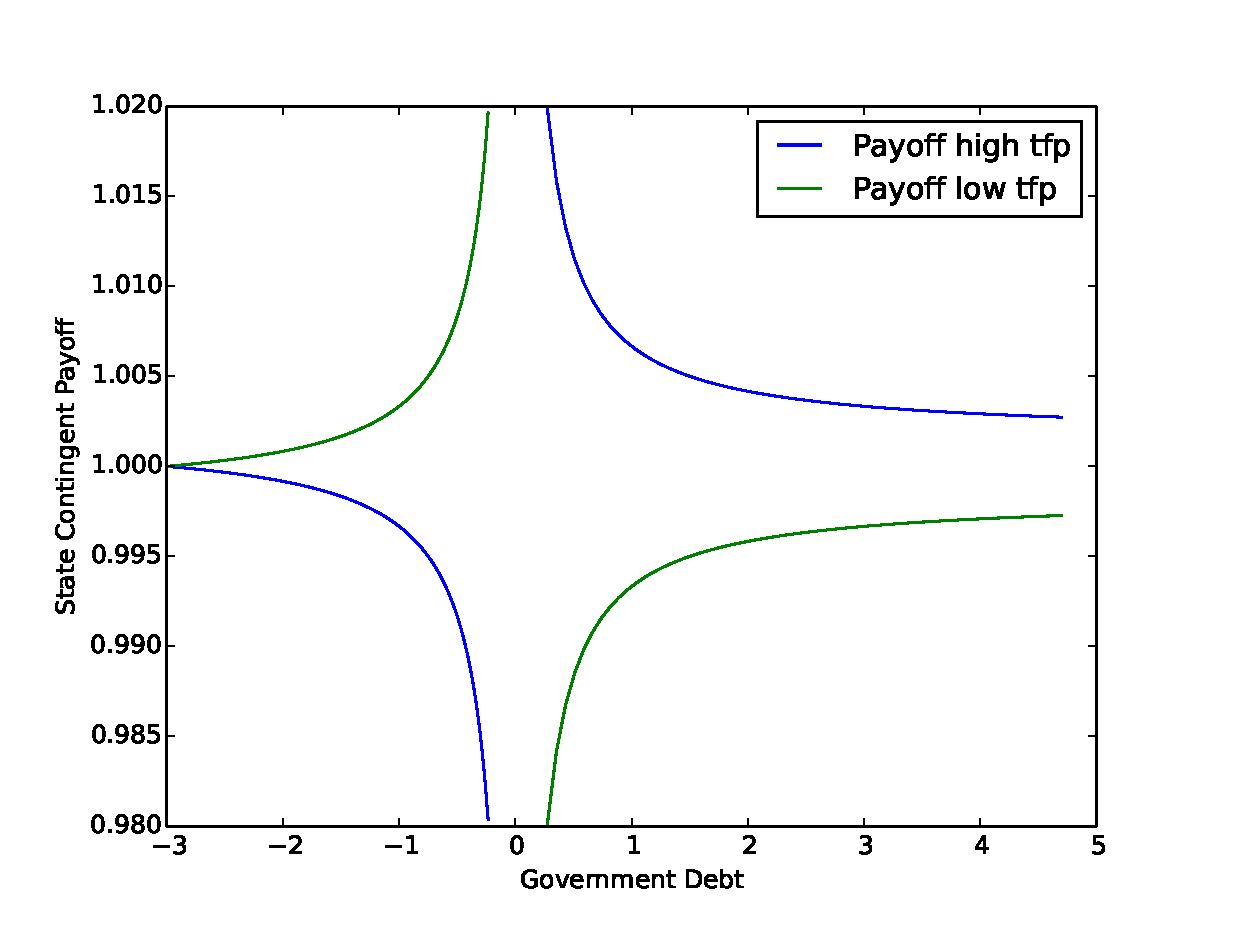
\includegraphics[scale=.35]{Images/p_graph_tfp.eps}
		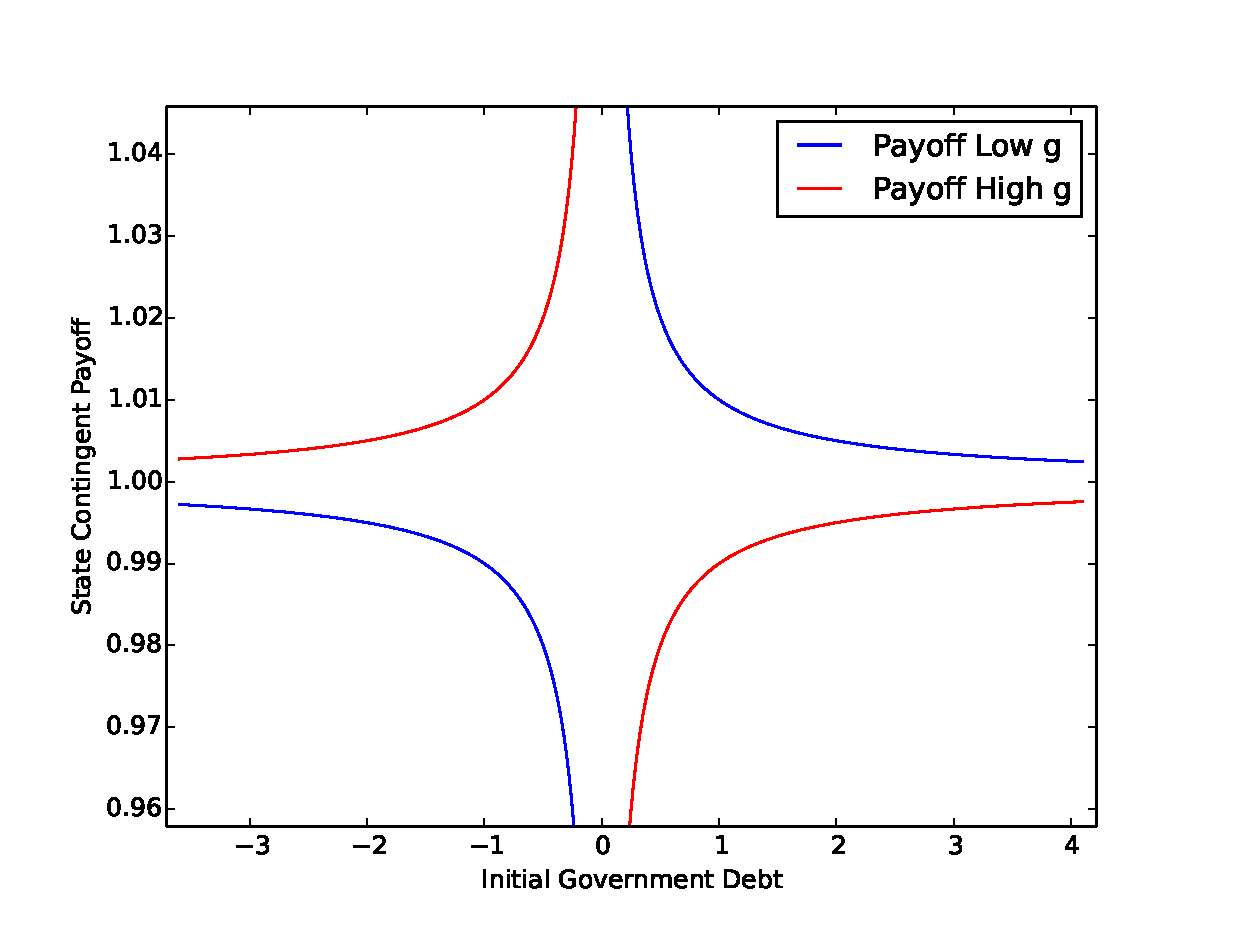
\includegraphics[scale=.35]{Images/p_graph.eps}
		\caption{Optimal asset payoff structure as a function of initial government debt when TFP follows a 2 shock i.i.d. process (left)
		and when government expenditures follow a 2 shock i.i.d process (right).\label{fig:optP}}
	\end{center}
\end{figure}


To appreciate how  the initial government debt level influences the optimal asset payoff structure via formula \eqref{eqn:optPP}, call a
 state $s$ ``adverse''  if it implies either ``high'' government expenditures or ``low '' TFP; formally, say that  $s$ is ``adverse'' if
\[   g(s)\EE \theta^\frac{\gamma}{1+\gamma}-\theta(s)^\frac\gamma{1+\gamma}\EE g >0\]
A ``good'' state is the opposite of an ``adverse'' state.  ``Adverse'' states have the property that for  wide range of initial government debts, the net-of-interest government surplus is lower than in ``good'' states.  When initial government assets are positive, \eqref{eqn:optPP} implies that  $\mathbb{P}^*$   pays {\em more} in ``adverse'' states, while when initial government assets are negative, $\mathbb{P}^*$  pays {\em less} in ``adverse'' states.

%
%\subsection{Inverting the $\mathbb{P}^*$ mapping}
%	\begin{enumerate}
%		\item  \textbf{Exogenous payoff structure:} Suppose $\mathbb{P}\neq \mathbb{P}^*(b_{-1})$
%
%		\item \textbf{Steady States: } A steady state is a government debt   $b^*$ such that
%		\[b_{t}=b^* \text{ implies } b_{t+\tau}=b^*\quad \forall \tau >0\]
%
%
%		\item \textbf{Characterization: } Given an asset payoff structure $\mathbb{P}$
%		\begin{itemize}
%			\item Does a steady state exist? Is it unique?
%			\item Value of $b^*$?
%			\item For what   \emph{initial government debts} $b_{-1}$ does  $b_t$ converge to $b^*$?
% 			\end{itemize}
%	\end{enumerate}

\subsection{The Inverse of $\mathbb P^*$ Again}\label{sec:David42} % $\mathbb{P}^{* -1}$}

Temporarily assume that $s_t$ is i.i.d and  $S=2$.  In this case, note that \eqref{eqn:optPP} implies that the optimal payoff matrix $\mathbb{P}^*$ has identical rows. This lets us restrict our attention to $\mathbb{P}(s,s\_)$ that have payoffs that are independent of $s\_$. This
 in turn lets us summarize  $\mathbb{P}$ with  a vector.
 Under the normalization  $\mathbb{E}\mathbb{P}(s)=1$, payoffs on the single asset are  determined by a  scalar $\bm{p}$, the payoff in state 1.   A risk-free bond is then a security for which $\bm{p} = 1$.  Without loss of generality, we shall assume that $ g(1)\EE\theta^\frac{\gamma}{1+\gamma}-\theta(1)^\frac\gamma{1+\gamma} \mathbb{E}g <0$, and thus, $\bm p$ is the payoff in the ``good'' state of the world.  Because the optimal payoff matrix can be summarized by a single scalar variable, we can recast the optimal matrix map $\mathbb P^*(b)$ as a single scalar function $\bm p^*(b)$.  The steady state level of debt associated with an exogenous  payoff $\bm p$ is then
\begin{equation}
\label{eq-ss}
 b^* =  {\bm p}^{* -1}(\bm{p}).
\end{equation}

\begin{proposition}\label{prop:ssexistence}
%\st{Suppose that $s$ shocks affect either $g$ or $\theta$.  Then there}\footnote{\dge{We don't need to assume either g or $\theta$ shocks as we have allready characterized what an adverse state of the world is}}
There exists $0 \geq \alpha_2\geq\alpha_1\geq1$
such that
  \begin{itemize}
   \item[a.] If $\bm{p}\leq \alpha_1$, then $b^* < 0$ % government holds assets in steady state
   \item[b.] If $\bm{p} \geq \alpha_2$, then $b^* > 0$ %government  issues debt  in steady state
   \item[c.] If $\alpha_1>\bm{p}>\alpha_2$, then $b^*$ solving \eqref{eq-ss}  does not exist
  \end{itemize}

\end{proposition}
\begin{proof}  Let $g_1$ and $\theta_1$ denote  government expenditures and TFP, respectively in the ``good'' state of the world.
% We begin by noting some facts about the complete markets solutionGGGGG.
%\st{
%As $(1-\tau)^\frac1\gamma\tau$ is maximized at $\frac\gamma{1+\gamma}$ there will be an upper bound for government debt for which a solution to the complete markets problem exists: $\overline b$.  This space of solutions to the complete markets problem can be indexed by $b\in(-\infty,\overline b]$.  If we let $\tau(b)$ the mapping from initial government debt into optimal tax rate, then $\tau$ is an increasing function of $b$ and $\tau((-\infty,\overline b]) = (-\infty,\frac{\gamma}{1+\gamma}]$.    Substituting $S(s,\tau)$ into equation we obtain}
 In state $s$, the government surplus is
\[
	S(s,\tau) = \theta(s)^\frac\gamma{1+\gamma}(1-\tau)^\frac1\gamma\tau - g(s),
\]  which  is  maximized at $\tau = \frac\gamma{1+\gamma}$ when $(1-\tau)^\frac1\gamma\tau$ is also maximized. Furthermore, in the region $(-\infty,\frac\gamma{1+\gamma}]$, $S(\cdot,\tau)$ is an increasing function of $\tau$.  In an i.i.d. world with complete markets, government debt
at a constant tax rate $\tau$ would be
\begin{equation}\label{eqn:tax_to_debt}
	\frac\beta{1-\beta} \sum_s \Pi(s) S(s,\tau),
\end{equation}which is an increasing function of $\tau$.  The maximal initial government debt sustainable with {\em complete} markets is then
\[
	\overline b^n = \frac1{1-\beta} \sum_s \Pi(s)\theta(s)^\frac\gamma{1+\gamma}\left(\frac{1}{1+\gamma}\right)^\frac1\gamma\frac{\gamma}{1+\gamma} - g(s) .\] Inverting the equation \eqref{eqn:tax_to_debt} mapping   from the tax rate into government debt gives us a function $\tau(b)$ that maps initial government debt into an optimal tax rate. The function $\tau(b)$ is an increasing function of $b$ on the domain of possible complete markets initial debts $(-\infty,\overline b^n]$, with $\tau((-\infty,\overline{b}^n]) = \left(-\infty,\frac\gamma{1+\gamma}\right]$.


Substituting the formula for $S(s,\tau)$ into equation \eqref{eqn:optPP}, we obtain
\[
	\bm p^*(\tau) = (1-\beta)\frac{\theta_1^\frac\gamma{1+\gamma}(1-\tau)^\frac1\gamma\tau-g_1}{\EE\theta^\frac\gamma{1+\gamma}(1-\tau)^\frac1\gamma\tau - \EE g} + \beta .
\]  Solving for $(1-\tau)^\frac1\gamma\tau$ gives
\[
	(1-\tau)^\frac{1}{\gamma}\tau = \frac{(\bm p^*-\beta)\EE g-(1-\beta)g_1}{(\bm p^* - \beta)\EE\theta^\frac{\gamma}{1+\gamma}-(1-\beta)\theta_1^\frac{\gamma}{1+\gamma}} .
\]  The set of complete market optimal tax rates is $(-\infty,\frac\gamma{1+\gamma}]$.  Since the mapping  $(1-\tau)^\frac1\gamma\tau$ is one to one
 and $b(\tau)$ is increasing on this domain, we conclude that $\bm p^*(b)$ is one to one. Differentiating $\bm p^*(\tau)$ with respect to $\tau$  yields
\[
	\frac{d}{d\tau} \bm p^*(\tau) = (1-\beta)(1-\tau)^{\frac1\gamma-1}\left[\gamma-(1+\gamma)\tau\right]\frac{g_1\EE\theta^\frac{\gamma}{1+\gamma}-\theta_1^\frac\gamma{1+\gamma}\EE g }{(\EE\theta^\frac\gamma{1+\gamma}(1-\tau)^\frac1\gamma\tau-\EE g)^2} <0,
\] implying that $\bm p^*(b)$ is decreasing in $b$. Since  $b =0$ implies that $\EE S(\tau(b)) =0$, the function function $\bm p^*(b)$ has a pole at $b = 0$.  That $\bm p^*(b)$ decreasing in $b$ must therefore imply that $\lim_{b\rightarrow0^{-} } \bm p^*(b) = -\infty$ and $\lim_{b\rightarrow 0^+} \bm p^*(b) = \infty$.  We conclude that
\[
	\bm p^*((-\infty,\overline b^n]) = \bm p^*((-\infty,0))\cup \bm p^*((0,\overline b]) = (-\infty,\alpha_1)\cup[\alpha_2,\infty).
\] We compute the bounds $\alpha_1$ and $\alpha_2$ by taking the limits of $\bm p^*$ as $b$ approaches $-\infty$ and the upper bound for government
debt under complete markets $\overline b$, or equivalently as $\tau$ approaches $-\infty$ and $\frac\gamma{1+\gamma}$, respectively.
\end{proof}
 With only government expenditure shocks, we compute
		\[
			\alpha_1 = 1 \text{  and }  \alpha_2 = (1-\beta)\frac{\theta^\frac{\gamma}{1+\gamma}\left(\frac{1}{1+\gamma}\right)^\frac1\gamma\frac{\gamma}{1+\gamma}-g(s_1)}{\theta^\frac{\gamma}{1+\gamma}\left(\frac{1}{1+\gamma}\right)^\frac1\gamma\frac{\gamma}{1+\gamma}-\EE g} +\beta>1
		\]
		With only TFP shocks, we compute
		\[
			\alpha_1 = (1-\beta)\frac{\theta(s_1)^\frac{\gamma}{1+\gamma}}{\EE\theta^\frac{\gamma}{1+\gamma}}+\beta > 1
		\]and
		\[
		\alpha_2 = (1-\beta)\frac{\theta(s_1)^\frac{\gamma}{1+\gamma}\left(\frac{1}{1+\gamma}\right)^\frac1\gamma\frac{\gamma}{1+\gamma}-g}{\EE\theta^\frac{\gamma}{1+\gamma}\left(\frac{1}{1+\gamma}\right)^\frac1\gamma\frac{\gamma}{1+\gamma}-g}+\beta>\alpha_1
		\]

\begin{remark}
		With only TFP shocks, the bond payoff has the special property that it is associated with a steady state asset level that supports the first-best allocation, $\bm p^{* -1}(1) = b_{fb}$.  At the first-best taxes are zero, so the net-of-interest government surplus is constant across states.
		\end{remark}
		We illustrate Proposition \ref{prop:ssexistence} in figure \ref{fig:noStable}.  The  blue curve is the inverse map $\bm p^{*-1}$.  Two constants $\alpha_1$ and $\alpha_2$ divide  possible payoff structures into three regions: one in which a steady state exists with the government holding assets,
another in which  a steady state exists with the government owing debt, and yet another in which  where a steady state does not exist.
		\begin{figure}[ht]
		\begin{center}
		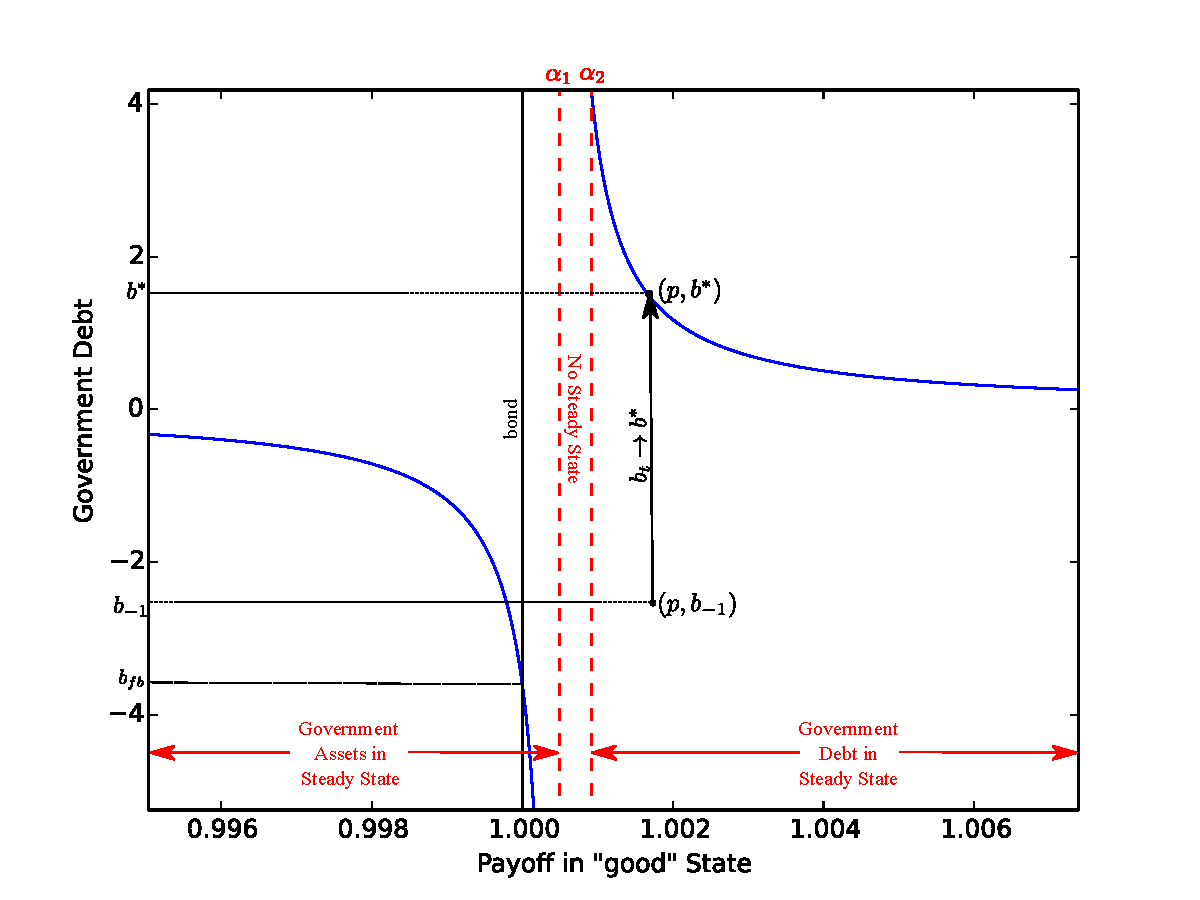
\includegraphics[width=5.5in]{Images/graph_nostable.pdf}
\caption{Three regions in $\bm{p}$ space.\label{fig:noStable}}
	\end{center}
	\end{figure}
\subsection{Long Run Assets} \label{sec:David43}
In subsection \ref{sec:David42},  we provided conditions under which there exists $b^*$ such $\bm p^*(b^*) = \bm p$.  By construction, if $b_{-1} = b^*$ then the allocation that solves complete markets Ramsey problem \ref{prob:RamseyLS} for initial condition $b^*$  automatically satisfies the measurability constraints \eqref{eqn:AMSSimplement}.  That allocation therefore solves the incomplete markets Ramsey problem \ref{prob:RamseyBEGS}.  This implies that if $b_{-1} = b^*$, then $b_t = b^*$ for all $t$.  Thus, $p^{*-1}(\bm p)$ corresponds to a ``steady state''.  It remains to be determined whether  the incomplete markets Ramsey $b_t$  converges to  $b^*$  for arbitrary $b_{-1}$.  Theorem \ref{thm:convergence} provides sufficient conditions for  convergence.


%\tjs{Tom stopped here at 11:30 pm Milan time on November 13}

 	\begin{theorem}\label{thm:convergence}
Let % $b^*$ denote steady state govt.  debt and
$b_{fb}$ denote the level of  government  debt associated with the first-best allocation with complete markets.
Then % for  same $  \alpha_1 < \alpha_2$
		\begin{itemize}
			\item[a.]  If $\bm{p}\leq\min(\alpha_1,1)$, then  $b_{fb}<b^*<0$ and $b_t\rightarrow b^*$ with probability 1.
			\item[b.] If $\bm{p} \geq \alpha_2$, then   $0<b^*$ and $b_t \rightarrow b^*$ with probability 1.
            \item[c.] If $ \min(\alpha_1,1)<\bm{p}<\alpha_2 $,   $b^*$ either does not exist or is unstable.
									\end{itemize}			\end{theorem}
  For $\bm{p}$ in region (c),
the government  run up debt over time.

\begin{proof}
%\dge{\st{The first order conditions governing the optimal allocation allow us to treat $\mu_t$ the multiplier on the measurability constraints as the state variable. }}
The optimal allocation can be represented recursively in terms of  functions $c_t(\mu_t),l_t(\mu_t), b_t(\mu_t)$ together  with a law of motion for $\mu' = \mu'(\mu,s)$ for $\mu$.
%\dge{
We shall establish show global stability under the assumption that $\mu'(\mu,s)$ an increasing function of $\mu$
% YYYYYYYY \footnote{\dge{ I'm still working on this.  I'm not sure if we'll need to include it as an assumption or not}}
The heart of the proof revolves around the twisted-martingale equation for $\mu$:
\[
	\mu_t = \sum_s \Pi(s) p_s \mu'(\mu_t,s) = \EE_t p_{t+1}\mu_{t+1}.
\]  We have shown that there is at most one $\mu^*$ such that $\mu'(\mu^*,s) = \mu^*$ for all $s$.  Here we focus on showing global stability for $\mu < \mu^*$. The twisted-martingale equation can be decomposed as follows
\[
	\mu_t = \EE_t \mu_{t+1}+Cov_t(p_{t+1},\mu_{t+1}).
\] By signing $Cov_t(p_{t+1},\mu_{t+1})$,  we can determine whether $\mu_t$ follows a sub or super-martingale.  Given that $\mu_t$ is bounded from above,\footnote{Since  $\mu'(\mu^*,s) = \mu^*$ and $\mu'(\mu,s)$ is increasing in $\mu$,  we know that if $\mu_t < \mu^*$, then $\mu_{t+j} < \mu^*$ for all histories $s^{t+j}$.} we can verify global convergence to the steady state if $\mu_t$ is a supermartingale.  As in the statement of the theorem, we will split the proof up into three cases. Recall that $\bm p$ is the payoff in the ``good'' state 1.
\begin{description}
	\item[1. $\bm p < \min\{1,\alpha_1\}$:]  Let $\overline b^n_s$ be maximal debt with which the government %\st{good}
 could enter a period and be able to pay off, assuming that  it  receives shock $s$ from this period onward. Then
	\[
	\overline b^n_s = \left(\frac{p_s}{\beta}-1\right)^{-1}\left(\theta_s^\frac{\gamma}{1+\gamma}\left(\frac1{1+\gamma}\right)^\frac1\gamma\frac\gamma{1+\gamma}-g_s\right)
	\] because the government maximizes tax revenue  by setting %the proportional tax
 $\tau$ to $\frac\gamma{1+\gamma}$. % \tjs{David and Anmol: please read the preceding sentence. It doesn't make sense to me.}
 For $\bm p <\alpha_2$, it is possible to show that $\overline b^n_1 > \overline b^n_2$, and thus the natural debt limit is attained under repetition of the ``adverse'' state.  This implies that $\lim_{\mu\rightarrow-\infty} b(\mu) = \overline b^n_2$ and  $\lim_{\mu\rightarrow-\infty} \mu'(\mu,2) = -\infty$.  In order for the period-by-period budget constraint
	\[
		\frac{p_s}{\beta}b(\mu) = S(\mu'(\mu,s))+b(\mu'(\mu,s))
	\] to be satisfied for all $s$, it must be true that $\lim_{\mu\rightarrow -\infty} \mu'(\mu,1) >-\infty$ (as $\overline b^n_1 > \overline b^n_2$).  Continuity of $\mu$ together with the uniqueness of the steady state $\mu^*$ then implies that $\mu'(\mu,1) > \mu'(\mu,2)$ for all $\mu < \mu^*$.
	$\bm p < 1$ implies that $p_1 < p_2$, allowing us to conclude that $Cov_t(p_{t+1},\mu_{t+1}) < 0$.  We then have that
	\[
		\mu_t < \EE_t\mu_{t+1}
	\] for $\mu_t < \mu^*$.  Since $\mu'(\mu,s)$ is increasing and  continuous, and since $\mu'(\mu^*,s) = \mu^*$, we can iterate on the policy functions to show that if $\mu_t < \mu^*$, then for all $j> 0$, we must have $\mu_{t+j} <\mu^*$.  Thus, if $\mu_t <\mu^*$, then $\mu_t$ is a supermartingale bounded from below. That implies  that $\mu_t\rightarrow \tilde\mu$ for some constant $\tilde\mu$ with probability 1.  Then  we
can use  the continuity of $\mu'(\mu,s)$ to show that
	\[
		\mu'(\tilde u,s) = \tilde \mu,
	\] implying that $\tilde \mu =\mu^*$, as $\mu^*$ is the unique steady state.  The steady state is then globally stable since $\mu_t \rightarrow \mu^*$ with probability 1.
	\item[2. $\bm p \geq \alpha_2$:]  Following the same approach used  in for case 1, we know for $\bm p > \alpha_2$ that $\overline b^n_1 < \overline b^n_2$, implying that the natural debt limit is attained under repetition of  the ``good'' state.  As in case 1,  by taking limits we obtain $\lim_{\mu\rightarrow-\infty} \mu'(\mu,1) = -\infty$ and $\lim_{\mu\rightarrow-\infty}\mu'(\mu,2) > -\infty$.  This implies that $\mu'(\mu,1) < \mu'(\mu,2)$, which along with $p_1 > p_2$ implies $Cov_t(p_{t+1},\mu_{t+1}) <0$.  As in case 1, we then have global stability of the steady state for $\mu_t < \mu^*$.
	\item[3. $\min(\alpha_1,1) < \bm p < \alpha_2$:]   In this case, either there exists a steady state if $1 < \bm p \leq \alpha_1$ or there does not exist a steady state.  In either case the analysis for case 1 implies that $\mu'(\mu,1) > \mu'(\mu,2)$ for $\mu < \mu ^*$.\footnote{When
 a steady state does not exist, take $\mu^*$ to be $\infty$.}  Since $\bm p >1$ implies that $p_1 > p_2$, we can  conclude that $Cov_t(p_{t+1},\mu_{t+1}) > 0$, implying that
	\[
		\mu_t > \EE_t \mu_{t+1}.
	\]We thus cannot apply the martingale convergence theorem, leaving open the possibility that the steady state is not stable.
 %will locally be unstable. \apb{??? We havent defined local stability? }
\end{description}
\end{proof}
\begin{remark}  Figure \ref{fig:stable} illustrates  Theorem \ref{thm:convergence}.  In addition to depicting values of $\bm p$ for which a steady state exists, it  also highlights  regions where a steady state is stable. The theorem asserts  that there exist $\bm p$ for which a steady state exists
but is unstable. % but economy will not converge to the steady state allocation in the long run.
\end{remark}
\begin{figure}[ht]
		\begin{center}
		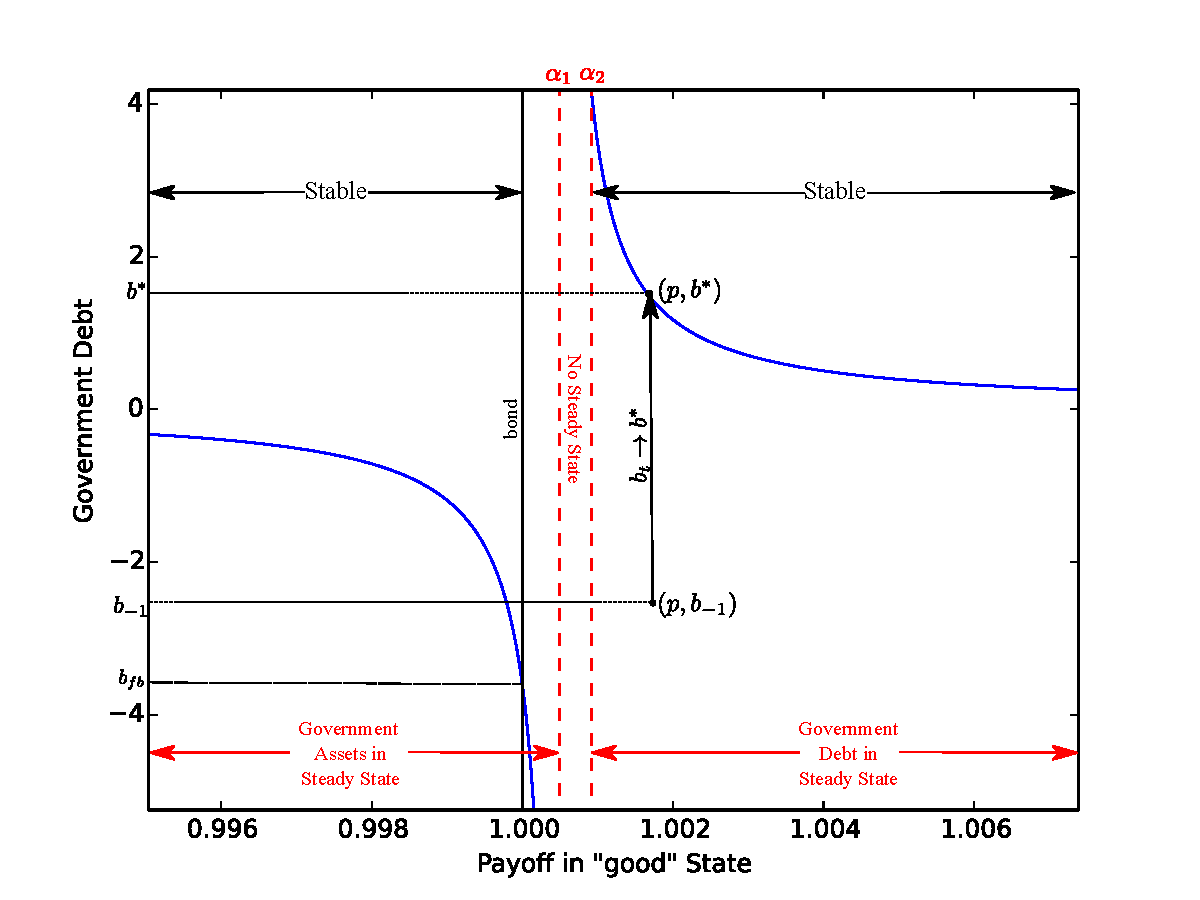
\includegraphics[width = 5in]{Images/graph_stable.pdf}
\caption{Stability regions in $\bm p$ space.\label{fig:stable}}
	\end{center}
\end{figure}  An important aspect of this model is that small changes in primitives (specifically $\bm p$) can lead to major differences in long run allocations.  To illustrate this, in Figure \ref{fig:2ps_figure} we plot two sample paths where the only difference is the asset restriction $\bm p$.
\begin{figure}
	\begin{center}
	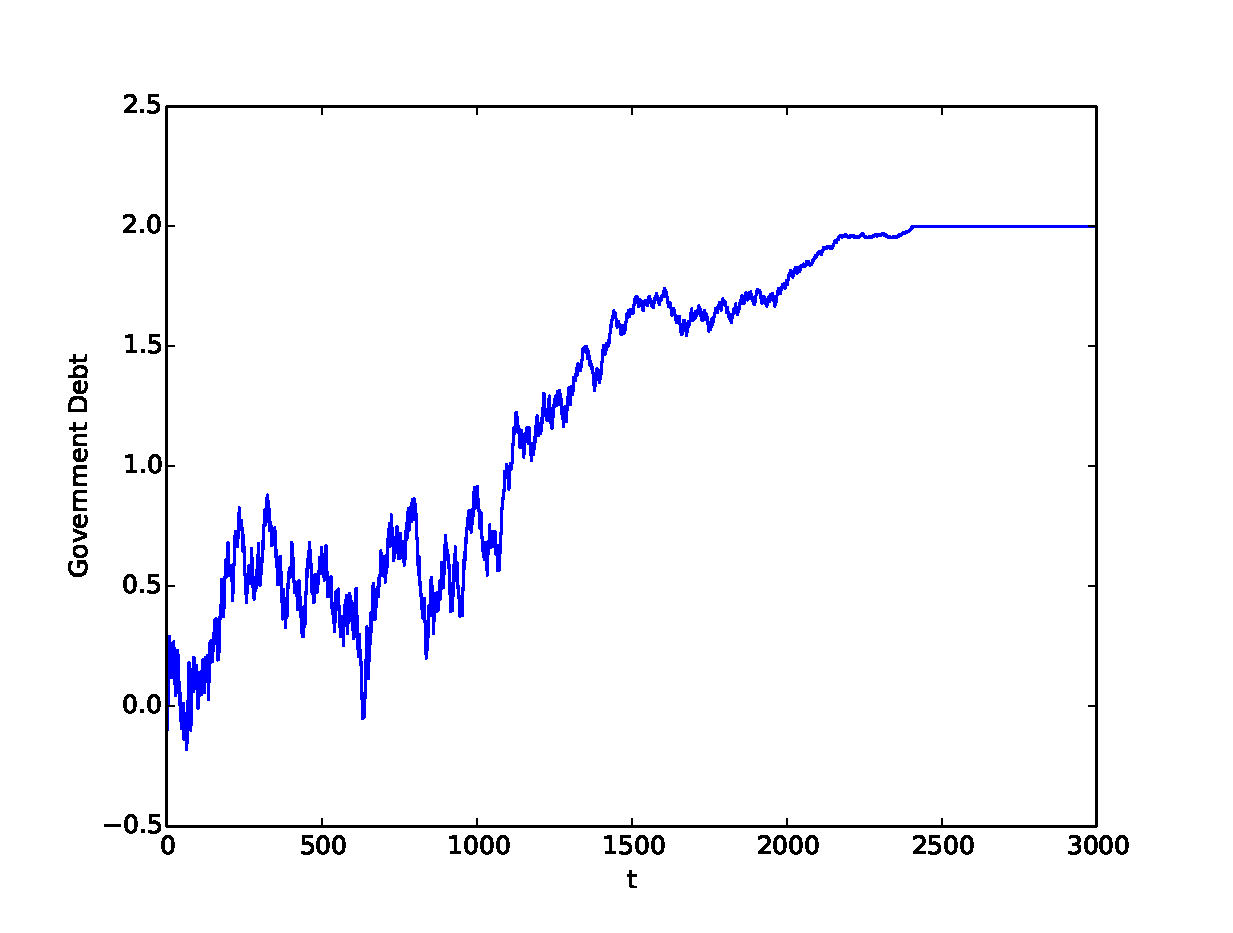
\includegraphics[width=3in]{Images/port1.eps}
	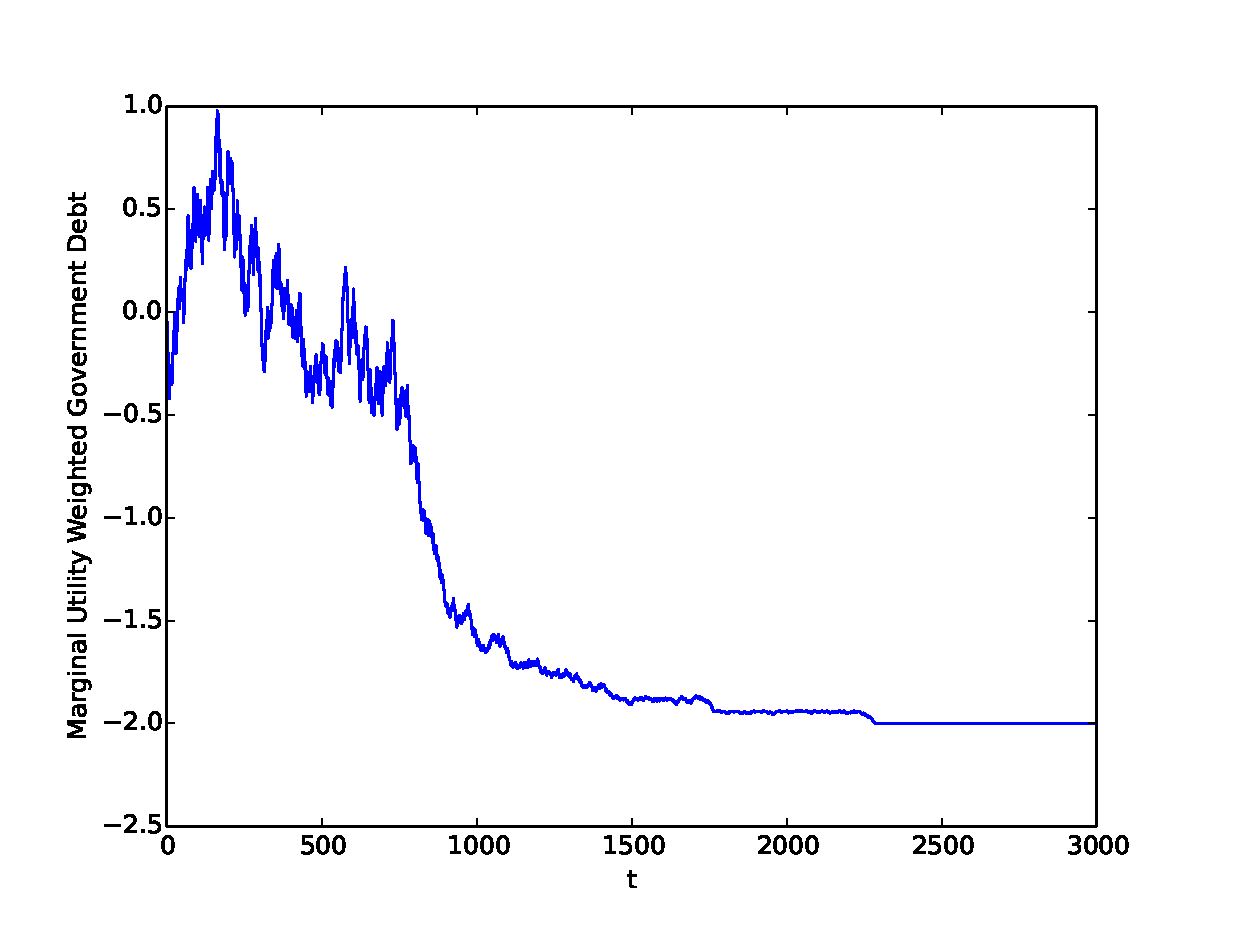
\includegraphics[width=3in]{Images/port2.eps}
\caption{A sample path with $\bm p > 1$ (left)  $\bm{p} <1$ (right).\label{fig:2ps_figure}}
	\end{center}
\end{figure}

\subsection{Economic forces driving convergence}
In summary, when the aggregate state follows a 2-state i.i.d. process, government debt  $b_t$ often converges to $b^*$, while
the tail of the allocation equals  Ramsey allocation for an economy with complete markets and initial government  debt $b^*$.
  The level  and sign of $b^*$ depend on the asset payoff structure, which we have  expressed in terms of a  scalar
  $\bm{p}$ that concisely captures what in more general settings we represented with the asset payoff matrix $\mathbb{P}$.


	  Facing incomplete markets, the  Ramsey planner recognizes that   the government's debt {\em level} combines with  the
 payoff structure on its debt instrument to affect  the welfare costs associated with varying the distorting labor tax rate across states.  When the
  instrument is a risk-free bond, the government's marginal cost of raising funds $\mu_t$ is  a martingale. In this situation,
    {\em changes} in debt levels  help smooth tax distortions across time.
	However, if the  payoff on the debt instrument varies across states, then  by affecting its state-contingent revenues, the {\em level} of government debt can help smooth tax distortions across states.
	For our two state, iid shock process,  the steady state debt level $b^*$, when it exists, is the unique amount of government debt
that provides just enough ``state contingency'' completely to fill the void left by  missing assets markets.  The Ramsey planner takes into account the additional benefits from tax smoothing as the government debt approaches $b^*$;  that puts a risk-adjustment into the martingale governing $\mu$ and leads the
 government either to accumulate or decumulate debt.
	 Although accumulating government assets requires  raising distorting  taxes, locally  the welfare costs of higher taxes are second-order and
so are  dominated by the welfare gains from approaching  $b^*$, which are first-order.

\section{More than Two Shocks}
Our analysis thus far has been limited to environments where there are two aggregate states of the world which are independently and identically distributed over time.  While we cannot solve analytically for the optimal policies for more general stochastic processes, we will show in this section how it is possible to obtain first order approximations to the optimal policy rules and compute the mean and variance of the ergodic distribution of the linearize system.  For this section we will restrict our attention to government expenditure shocks.   We set aggregate productivity, $\theta$, to be constant and normalize to one.  We allow exogenous government expenditure to take $S$ possible values which are i.i.d. over time with probability of government expenditure $g_s$  being $\mathbb P_s$. 

In order to approximate the optimal policies we need to linearize around a steady state.  The standard approach is to linearize around the non-stochastic steady state as the size of the shocks approaches zero.  We have found for this planning problem this approach does not accurately characterize the decision rules of the non-linear system\footnote{When linearizing around the steady state as the size of the shocks approaches zero, we find that the marginal value of debt $\mu_t$ is a martingale.  A key property of the policy rules for $\mu_t$ that produces the degenerate distribution of debt is that $\mu_t$ is a sub-martingale for sufficiently small $\mu_t$ and super-martingale for sufficiently large $\mu_t$.}.  Instead, we propose an alternative method utilizing the complete market steady states of the previous section.

We will show that if the payoff vector $\overline{\bm p}$ is perfectly correlated with government debt then there exists a complete markets Ramsey allocation that is a solution to the incomplete markets planning problem with payoff vector $\overline{\bm p}$.  The sign and magnitude of the covariance of $\overline {\bm p}$ with the government expenditure shock will determine the sign and magnitude of government debt in this allocation.  Given that the state variable $\overline b$, government debt, is constant under this allocation we can linearize the policy rules with respect to both government debt and payoff vector, allowing us to approximate the incomplete market policy rules at some pair $(b,\bm p)$ near $(\overline b,\overline {\bm p})$.  In fact, we will show that the best choice of $(\overline b,\overline{\bm p})$ is to minimize the distance
\begin{equation}\label{eq.p_norm}
	\| \bm p -\overline{\bm p}\|^2 = \sum_s \mathbb P_s (p_s -\overline p_s)^2
\end{equation} as then ergodic distribution of the linearized system will be centered around $\overline b$.

\subsection{Steady State Payoff Vectors}

Our first task is to find the set of payoff vectors, $\overline {\bm p}$ for which a complete markets allocation is a solution to the incomplete markets planning problem.  In Lemma \ref{lem.cm_payoff} we show that these payoff vectors must be perfectly correlated with $g$:
\begin{lemma}\label{lem.cm_payoff}
	 The payoff vector $\overline{\bm p}$, normalized so that $\EE\overline{\bm p} = 1$, associated with complete markets Ramsey allocation with government debt $\overline b \leq \overline b^n$ ($\overline b^n$ is the natural debt limit) must satisfy
	\begin{equation}\label{eq.pbar}
		\overline p_s = 1- \frac{\beta}{\overline b}(g_s - \EE g).
	\end{equation}Moreover, the steady state $\overline b$ is globally stable: $b_t\rightarrow \overline b$ with probability 1.
\end{lemma}  The proof of this Lemma is included in the Appendix, but the intuition is straightforward.  The complete markets allocation must have a constant tax rate $\overline \tau$.  The government surplus in state $s$, $S(\overline \tau,s)$, is then made up of two components: tax income $I(\overline \tau)$, which is independent of $s$, and government expenditure $-g_s$.  Income from government debt $\frac{\overline b}{\beta} \overline p_s$, must perfectly account for fluctuations in government surplus: $-g_s$.  Thus, $\overline{\bm p}$ must be perfectly correlated with the exogenous government expenditure process $g_s$.

Rearranging equation \eqref{eq.pbar}, and taking the covariance with respect to $g$ we see that if $\overline{\bm p}$ is perfectly correlated with government expenditures the associated level of steady state debt is
\[
	\overline b = -\beta \frac{\var(\bm g)}{\cov(\overline{\bm p},\bm g)}
\]The covariance of $\overline{\bm p}$ with $\bm g$ relative to the variance of government expenditure determines the level of steady state government debt, and the sign of the covariance determines if the government holds debt or assets in the steady state.  As before, the government is using fluctuating payments on debt to smooth tax rates.  If payoffs are perfectly correlated with good fiscal times (low $g$) then the government will hold debt in long run.  If payoffs are correlated with hard fiscal (high $g$) times then the government will hold assets.
\subsection{Ergodic Distribution of Linearized Policy Rules}
With the previous section we are able to complete characterize the ergodic distribution of global policy rules for a one-dimensional subspace of the space of all payoff vectors $\mathbb R^{S-1}$ (dimension $S-1$ after normalizing $\EE\bm p = 1$).  For $\bm p$ which are not perfectly correlated with $\bm g$ we can compute the mean and variance of the ergodic distribution of the linearized policy rules.  Any payoff vector $\bm p$, with $\EE\bm p =1$, can be uniquely decomposed into two components:
\[
	\bm p = \hat{\bm p} +\overline{\bm p}
\] where $\overline{\bm p}$ is perfectly correlated to $\bm g$ and $\hat{\bm p}$ is orthogonal to $\bm g$.  This is equivalent to finding $\overline{\bm p}$, perfectly correlated with $\bm g$, that minimizes  $\|\bm p-\overline{\bm p}\|^2$ in equation \eqref{eq.p_norm}.  Proposition \ref{prop.erg_lin} below then tells us that the ergodic distribution of government debt of the linearized policy rules will be centered around the steady state level of debt, $\overline b$, associated with $\overline{\bm p}$
\begin{proposition}\label{prop.erg_lin}
Suppose $\bm p$ admits a decomposition $\bm p = \hat{\bm p} +\overline{\bm p}$ with $\hat{\bm p}$ orthogonal to $\bm g$ and
\[
	\overline{\bm p} = 1- \frac{\beta}{\overline b}(\bm g - \EE g).
\] with $\overline b \leq \overline b^n$.  Then the ergodic distribution of debt of the policy rules linearized around $(\overline b, \overline{\bm p})$ will have mean $\overline b$ and variance
\begin{equation}\label{eq.var_lin}
	\frac{\overline b^2 \var(\hat{\bm p})}{\EE[\overline{\bm p}^2]\var(\overline{\bm p})}.
\end{equation}
\end{proposition}  The proof of this proposition is included in the appendix.  From Proposition \ref{prop.erg_lin}  we see that the location of the ergodic distribution of debt for the incomplete markets Ramsey allocation will be determined by the covariance of $\bm p$ and $\bm g$.  Specifically, since $\cov(\bm p,\bm g) = \cov(\overline{\bm p},\bm g)$, the ergodic distribution of the linearized policy rules will be centered around
\[
	 -\beta \frac{\var(\bm g)}{\cov(\overline{\bm p},\bm g)} =  -\beta \frac{\var(\bm g)}{\cov(\bm p,\bm g)}.
\]  We can also use equation \eqref{eq.var_lin} to quickly bound the variation of linearized system.  Rearranging terms and noting that $\EE[\overline{\bm p}^2] \geq 1$ we can bound the coefficient of variation of the ergodic distribution of the linearized policy rules
\begin{equation}
	\frac{\sigma_b}{\overline b} \leq \sqrt\frac{\var(\hat{\bm p})}{\var(\overline{\bm p})}
\end{equation}  The spread of the ergodic distribution relative to its mean is bounded by the loading of the payoff vector $\bm p$ on the component orthogonal to $\bm g$ relative to the loading on the component parallel to $\bm g$.
\section{Turning on risk-aversion}

  We now depart from quasi-linearity of $U(c,l)$ and thus activate an additional source of return fluctuations coming from endogenous fluctuations in prices of the asset $q_t$.  To obtain a recursive representation of a Ramsey plan,
  we employ the endogenous state variable
  \[x_t=u_{c,t}b_{t} ,\]
  and study how long-run properties of $x_t$ depend on equilibrium returns $R_{t,t+1}=\frac{\mathbb{P}(s_t,s_{t+1})}{q_t(s^t)}$.
   Activating risk aversion in consumption makes $q_t$ vary in interesting ways.

  Commitment to a Ramsey plan implies that government actions at $t \geq 1$ are constrained by the household's anticipations about them at $s < t$
	 Following \citet{Kydland1980}, we  use the  marginal utility of consumption that the
Ramsey planner promises to the household to account for that `forward looking' restriction on the Ramsey planner. That
comes from the fact that the Euler equation restricts allocations such that expected marginal utility in time $t$ is constrained by consumption choices
in time $t-1$.  It is convenient for us that scaling the household's  budget constraint by the  marginal utility
 of consumption makes Ramsey problem  recursive in  $x=U_c b$.  In particular, implementability constraints \eqref{eqn:AMSSimplement}
 can be represented as
		\begin{equation}
		\frac{x_{t-1} \mathbb{P}(s_t,s_{t-1}) U_{c,t}}{\beta \EE_{t-1} \mathbb{P}U_{c,t}}  = U_{c,t}c_t+U_{l,t} l_t + x_t, \ t \geq 1
	\end{equation}

\begin{problem}\label{prob:RamseyBellman}
% Before the realization of the time $t$ Markov shock $s_t$,
Let   $V(x, s_{-1})$ be the {\em expected} continuation value of the Ramsey plan at $t \geq 1$  given promised marginal utility government debt inherited
from the past $x = U_{c,t} b_t $ and time $t-1$ Markov state $s_{-1}$.
After the realization of time $0$ Markov shock $s_0$, let $W(b_{-1},s_0)$ be the value of the Ramsey plan when initial
government debt is $b_{-1}$. % These value functions satisfy  two
%Bellman equations.
The (\textit{ex ante}) Bellman equation for $t\geq1$  is
	\begin{equation}\label{eqn:Bellman1}
		V(x,s\_) = \max_{c(s),l(s),x'(s)} \sum_s \Pi(s,s\_)\Bigl(U(c(s),l(s)) + \beta V(x'(s),s)\Bigr)
	\end{equation}
subject to $x'(s)\in [\underline x,\overline x]$ and
	\begin{align}
		\frac{x \mathbb{P}(s,s\_) U_c(s)}{\beta\EE_{s\_} \mathbb{P}U_c} =U_c(s)c(s)+U_l(s)l(s) + x'(s) \label{timetBellimplement}\\
		c(s) + g(s) = \theta(s)l(s) \label{timetfeas}
	\end{align}
Equation \eqref{timetBellimplement} is the implementability constraint and \eqref{timetfeas} is feasibility.
	Given an initial  debt $b_{-1}$,time $0$ Markov state $s_0$,  and continuation value function $V(x,s\_)$, the (\textit{ex post}) time $0$ Bellman equation is
%\tjs{Anmol and David XXXXX: I altered the below by adding the $W$ function; but there is a problem with the timing of
%the $b$ argument.  See earlier slide where $W$ is defined.}
	\begin{equation}\label{eqn:Bellman0}
		W(b_{-1},s_0) = \max_{c_{0},l_0,x_{0}} U(c,l) +\beta V(x_0,s0)
	\end{equation} subject to  time zero implementability constraint
	\[
		U_{c}(c_0,l_0)c + U_l(c_0,l_0) l_0 + x_0 = U_c(c_0,l_0) b_{-1}
	\]and  the resource constraint
	\[
		c_0+ g(s_0) = \theta(s_0) l_0
	\]and
	\[
		x_0 \in [\underline x,\overline x]
	\]
\end{problem}
\begin{lemma}  Let $V, W$ be the optimal value functions for  problem \ref{prob:RamseyBellman}.  The allocation given by the  corresponding optimal policy function solves problem \ref{prob:RamseyBEGS}.
\end{lemma}

\subsection{Computational and analytic strategy}

% \tjs{David and Anmol XXXXXX: please edit and add to this section. A brief paragraph describing the computational strategy and a reference to an appendix, perhaps
% separate from the paper, is all that are needed.}
The analysis in this section is based on two pillars: (1) a suite of \texttt{python} computer programs that solves Bellman equations
\eqref{eqn:Bellman1} and \eqref{eqn:Bellman0}; and (2) some mathematical analysis of first-order conditions satisfied by
the  optimal policy function that attain the right sides of these Bellman equations.
% As for pillar 1, we approximate the value function $U, V$ by XXXXX and the policy rules by XXXXX.
% \tjs{David and Anmol XXXXX: please complete the above sentence and paragraph. Please add a remark or two foretelling some of the analysis to come. You can be brief.}

We attacked Ramsey  Problem \ref{prob:RamseyBellman} with two weapons: (1) a suite of \texttt{python} computer programs that solve Bellman equations \eqref{eqn:Bellman1} and \eqref{eqn:Bellman0};
and (2) mathematical analysis of the first-order conditions satisfied by the optimal policy functions that attain $U$ and $V$. In our computational approach,
we solved the Bellman equations via policy iteration on  first-order conditions.  Appendix \ref{sec:app_numerical} tells how we take $V_x(x,s\_) = \tilde{\mu}$ as a state variable
and approximate the optimal policy  $x(\tilde \mu,s\_)$ with quadratic splines.\footnote{We also solved the
problem numerically using value function iteration.  Numerical expriments showed that policy function iteration provided more accurate and stable solutions.}
As with the quasilinear section, our analytical approach is confined to environments with a two state i.i.d. process for  the aggregate state $s_t$.
We use our numerically computed optimal policy functions to confirm that much  of the  intuition  acquired from our formal mathematical analysis of the two-state, i.i.d.\ process
extends to  general stochastic processes for $s_t$.

\subsection{Motivation to focus on risk-free bond economy\label{sec:riskfreeonly}}

As mentioned in section \ref{sec:excusequasilinear},  properties of a Ramsey plan for our incomplete markets economy vary sensitively  with   asset returns that reflect
	properties of equilibrium prices $\{q_t(s^t|B_{-1},s_{-1})\}_t$ and the exogenous asset payoff matrix $\mathbb{P}$.  By studying
quasi-linear preferences, we eliminated fluctuations in returns coming from prices.  Here we turn the table and by studying an economy
with a risk-free bond, we eliminate fluctuations in returns coming from the exogenous asset payoff matrix $\mathbb{P}$.
Thus, we set $\mathbb{P}(s|s\_)=1 \ \forall \ (s,s\_)$.



Let $x'\left( s;{x},s\_\right) $ be the decision rule for $x'$ that attains the right side of the $t\geq1$ Bellman equation
\eqref{eqn:Bellman1}.  A steady state  ${x}^{*} $  satisfies ${ x}^{*}  =x' \left( s;{x}^{*},s_{-}\right) $ for all $%
\,s,s\_$.
A steady state is a node at which the  continuation allocation and tax rate have no further history dependence.

\begin{proposition}\label{prop:existenceU}
Assume that $U$ is  separable and iso-elastic,	 $U(c,l) = \frac{c^{1-\sigma}}{1-\sigma} -\frac{ l^{1+\gamma}}{1+\gamma}$.
Assume that

%\apb{XXXX We are changing notation to represent good states with $s=s_g$ instead of $s=1$ ?}

	 the Markov state $s$ take two values is  i.i.d with $s_b$  being the ``adverse'' state (either low TFP or high govt. expenditures)
and $s_g$ begin the good state.
		Let $x_{fb}$ be the discounted present value of marginal utility weighted government surpluses associated with the first best allocation.
%\st{ be a value of  %\st{the state $x$ from which a government can implement first=best with complete markets}
%marginal utility weighted debt associated with the first-best allocation with complete markets.}\tjs{David: the phrase
%``first-best allocation with complete markets'' remains imprecise?  What does it mean?}
	 Let $q_{fb}(s)$ be the shadow price of government debt in state $s$ at the first best allocation.
	If
	\begin{equation}\label{eqn:prop52sufficient}
		\frac{1-q_{fb}(s_b)}{1-q_{fb}(s_g)} > \frac{g(s_b)}{g(s_g)}\geq 1 ,
	\end{equation}
		then there exists a steady state with $x_{fb}>x^*>0$
		\end{proposition}

\begin{proof}As in the quasi-linear case, a steady state is associated with a continuation allocation of a complete markets allocation starting from  some initial debt level.  We can index such continuation allocations by their associated multiplier $\mu$ on the implementability constraint.  Letting $S(\mu,s)$ be the government surplus at state $s$ and multiplier $\mu$, a steady state has  a multiplier $\mu^*$ at which the budget constraint in both states of the world is satisfied:
\[
	\frac{S(\mu^*,s_g)}{\frac{c(\mu^*,s_g)^{-\sigma}}{\beta \EE c(\mu^*)^{-\sigma}}-1} =\frac{S(\mu^*,s_b)}{\frac{c(\mu^*,s_b)^{-\sigma}}{\beta \EE c(\mu^*)^{-\sigma}}-1}.
\]  By choosing $\mu_1$ so that $S(\mu_1,s_g) =0$, we conclude that
\[
	0 = \frac{S(\mu_1,s_g)}{\frac{c(\mu_1,s_g)^{-\sigma}}{\beta \EE c(\mu_1)^{-\sigma}}-1} > \frac{S(\mu_1,s_b)}{\frac{c(\mu_1,s_b)^{-\sigma}}{\beta \EE c(\mu_1)^{-\sigma}}-1}.
\]  We derived this equation directly from $S(\mu,s_g) < S(\mu,s_b)$ for all $\mu$ and $c(\mu,s_g) > c(\mu,s_b)$ for all $\mu$.

Eliminating  $q_{fb}$, equation \eqref{eqn:prop52sufficient} can expressed as
\[
	\frac{g(s_g)}{1-\frac{\beta\EE c_{fb}^{-\sigma}}{c_{fb}(s_g)^{-\sigma}}} > \frac{g(s_b)}{1-\frac{\beta\EE c_{fb}^{-\sigma}}{c_{fb}(s_b)^{-\sigma}}}.
\]  Multiplying both sides by $-1$ and factoring out  $\beta\EE c_{fb}^{-\sigma}$, this equation simplifies to
\[
	\frac{-c_{fb}(s_g)^{-\sigma}g(s_g) }{\frac{c_{fb}(s_g)^{-\sigma}}{\beta \EE c_{fb}^{-\sigma}}-1} < \frac{-c_{fb}(s_b)^{-\sigma}g(s_b) }{\frac{c_{fb}(s_b)^{-\sigma}}{\beta \EE c_{fb}^{-\sigma}}-1}
\]or
\[
	\frac{S(0,s_g)}{\frac{c(0,s_g)^{-\sigma}}{\beta \EE c(0)^{-\sigma}}-1} <\frac{S(0,s_b)}{\frac{c(0,s_b)^{-\sigma}}{\beta \EE c(0)^{-\sigma}}-1}.
\]  Existence of $\mu^*$ follows directly from the Intermediate Value Theorem.
\end{proof}


	\begin{proposition}\label{prop:convergenceU}
%\st{ Let $\{c_t(s^t), l_t(s^t), x_t(s^{t-1})\}$ solve the incomplete markets Ramsey problem with $x_0 > x^*$.  Then  $x_t(s^{t-1})\rightarrow x^*$ as $t\rightarrow \infty$ with probability 1 for all initial conditions.}
  There exist $\underline x < x^*$ and $\overline x >0$ such that if $\{c_t(s^t), l_t(s^t), x_t(s^{t-1})\}$ solves the incomplete markets Ramsey problem \ref{prob:RamseyBellman} with bounds $\underline x$ and $\overline x$, then $x_t(s^t)\rightarrow x^*$ as $t\rightarrow\infty$ with probability 1.

	\end{proposition}


\begin{proof}  {The proof relies on the concavity of the value function $V$ and  two lemmas  that describe the structure of the policy functions.  Proofs of
 the lemmas appear in the appendix.
\begin{lemma}\label{lem:c_order}  Consumption is ordered by the state of the world.  In particular, there exist $\underline x$ and $\overline x$ such that for all $x\in[\underline x,\overline x]$, the policy function for consumption satisfies $c(x,s_g) > c(x,s_b)$.
\end{lemma}  This lemma assures that for the same level of marginal utility weighted government debt, consumption is larger in ``good'' states of the world than in ``adverse'' states of the world.
\begin{lemma}\label{lem:x_order}  There exist $\underline x$ and $\overline x$ such that the optimal government savings policy $x'(x,s)$ satisfies
\begin{enumerate}
	\item For $x\in(x^*,\overline x]$, $x'(x,s_g) < x'(x,s_b)$
	\item  For $x\in[\underline x, x^*)$, $x'(x,s_g) > x'(x,s_b)$
\end{enumerate}  Furthermore, $x'(x,\cdot)$ is increasing in $x$.
\end{lemma}  Property 1 states that if government debt exceeds its steady state value, then the government issues more debt in bad states of the world than in good states of the world.  Property 2 states that if government debt is smaller than its  steady state amount, then the government
has accumulated enough assets that
the lower interest rate in the ``adverse'' state of the world allow it to purchase more assets (issue less debt) than in the ``good'' states of the world.\footnote{Remember that  in the steady state, the government  owns a positive amount of the risk-free asset.}     The last part of the lemma guarantees that if the government enters with more debt, it will pass on more debt to future periods.  We can now prove global convergence. We will focus on the case where $x_t \geq x^*$, since the analysis of the other case is symmetric. Since $x'(x,\cdot)$ is increasing in $x$, we can iterate the policy functions forward to conclude that $x_{t+j} > x^*$ for all $j$ as long as $x_t >x ^*$.  Letting $\mu_t = V'(x_t)$ be the multiplier on the
implementability constraint and $\overline \lambda_t$ be the multiplier on the constraint $x_t \leq \overline x$, we have
\[
	 \mu_t = \frac{1}{\EE_t[c_{t+1}^{-\sigma}]}\EE_t[\mu_{t+1}c_{t+1}^{-\sigma}] -\overline \lambda_t
\]  Lemma  \ref{lem:x_order}. along with concavity of $V$ allows us to conclude that $\mu_{t+1}(s_g) > \mu_{t+1}(s_b)$.  From Lemma \ref{lem:c_order}, we know that $c_{t+1}(s_g) > c_{t+1}(s_b)$, which implies that $Cov_t(\mu_{t+1},c_{t+1}^{-\sigma}) <0$, so
\[
	 \frac{1}{\EE_t[c_{t+1}^{-\sigma}]}\EE_t[\mu_{t+1}c_{t+1}^{-\sigma}]  < \EE_t[\mu_{t+1}].
\] Since $\overline \lambda_t \geq 0$, we  conclude that
\[
	\mu_t < \EE_t[\mu_{t+1}].
\]  Moreover $\mu_t < V'(x^*) = \mu^*$, so $\mu_t$ is a submartingale that is bounded from above.  Applying the martingale convergence theorem, we conclude that $\mu_t \rightarrow \mu^*$ with probability 1.  Continuity of the policy functions and uniqueness of the steady state in the region $[x^*,\overline x]$ implies that $x_t\rightarrow x^*$ with probability 1.}
\end{proof}

\begin{remark}
In this economy,  fluctuations in the risk-free  interest rate come from fluctuations in  marginal utility of consumption. The interest rate
 is low  in ``good'' states (i.e., when  TFP is high or government expenditures are low).
 In a steady state, the government holds claims against the private sector, an outcome that resembles those in economies
 with  quasi-linear utility and  low  $\bm{p}$.  For all admissible  initial  levels of government debt, an incomplete markets Ramsey allocation converges to a particular Lucas-Stokey  Ramsey allocation.
%\tjs{Team xXXXXX: say a little more about the particular LS allocation and its initial debt level}

%\tjs{Stopped here on plane GGGG}
\end{remark}
{
\begin{remark}  Propositions \ref{prop:existenceU}  and \ref{prop:convergenceU} should be interpreted approximately as supplying  a converse to Lemma 3 from section 5 of \citet{Aiyagari2002}, which  provided sufficient conditions for their incomplete markets Ramsey plan  economy to {\em fail} to converge to  a complete markets continuation allocation.  Our propositions \ref{prop:existenceU}  and \ref{prop:convergenceU} provide sufficient conditions for a complete markets steady state continuation allocation to exist, and for the incomplete market Ramsey allocation to converge
%\st{to that
%the long rung convergence}\dge{, in the long run,}
to that steady state continuation allocation.  %While we don't challenge the \citet{Aiyagari2002} counterexamples to convergence,  do hold,
Note that propositions \ref{prop:existenceU}  and \ref{prop:convergenceU} assume a very special stochastic process for $s$.
  For more general stochastic processes, a steady state does not exist. But in simulations,  we have found that the outcomes described in Propositions \ref{prop:existenceU}  and \ref{prop:convergenceU} do a good job of approximating long run  dynamics of incomplete markets Ramsey plans for
 richer shock stochastic processes, in the sense that they converge to regions of low volatility.
\end{remark}}
Figure \ref{fig:conv_RA} plots a simulation of the Ramsey plan.  The path of marginal utility weighted government debt resembles the path of government debt for the quasilinear economy with low $\bm p$ plotted earlier in Figure \ref{fig:2ps_figure}.
\begin{figure}[ht]
	\begin{center}
	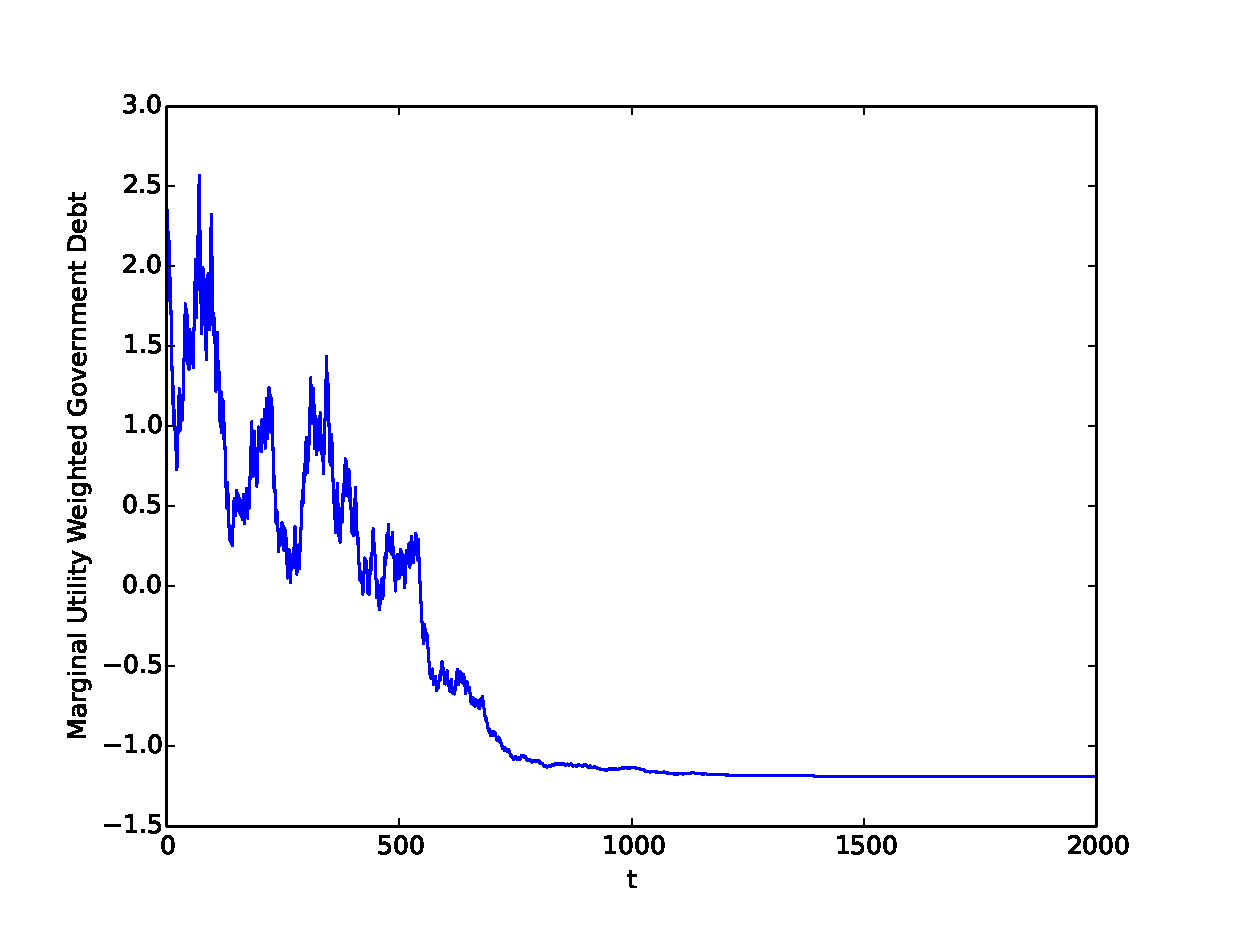
\includegraphics[width=4in]{Images/2stateiid.eps}
\caption{Sample path of $x_t$  for an economy with risk aversion and a 2 state i.i.d. process for TFP.\label{fig:conv_RA}}
	\end{center}
\end{figure}

%\tjs{Team XXXXXX: let's add some modest self-promotion here telling just how much the results immediately above add in terms of
%filling in loose ends from AMSS -- things they just weren't able to answer.}


% \section{To do}
%
% \begin{enumerate}
% \item Add above at appropriate place that until now $T_t \equiv 0$.
%
% % \item Tom to write introduction and concluding sections.
% % \item Fill in some notation about what objects are indexed by, e.g., $s^t$.
% % \item Fill in proofs.
% % \item Check flow and order.
%
% \end{enumerate}


\subsection{Allowing nonnegative transfers}
\begin{figure}[h]
	\begin{center}
	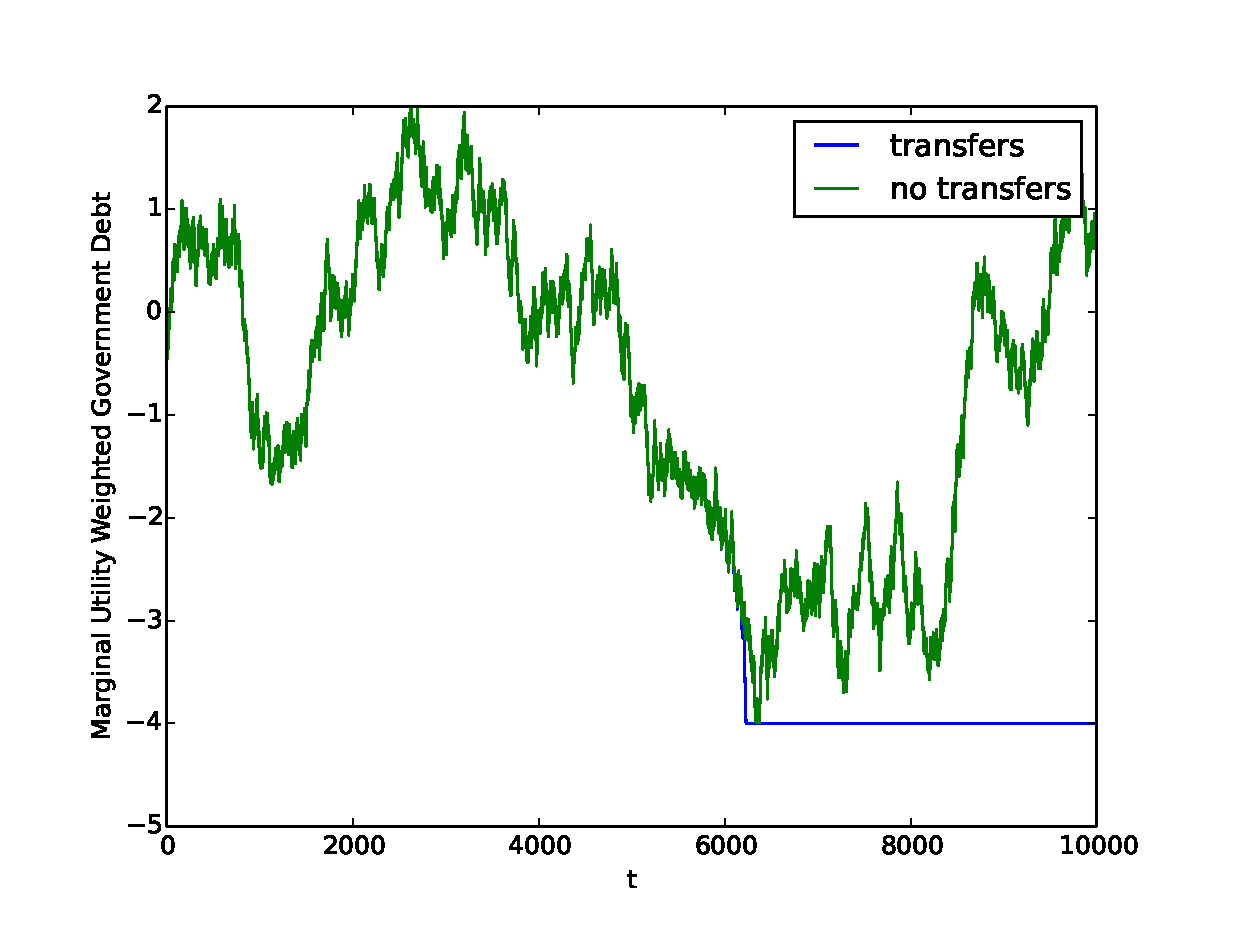
\includegraphics[width=4in]{Images/transfer_example2.eps}
\caption{Government  debt for two otherwise identical economies with quasilinear preferences and a risk-free bond, one economy   with nonnegative transfers, the other with zero transfers.\label{fig:nonnegative_transfers}}
	\end{center}
\end{figure}
% \tjs{David: let's write a tentative version of this section together. We can coordinate by phone or skype or in person.
% Add BS about AMSS and what transfers did for them. Write front end of this section -- good low-skill job for Tom.}
	Figure \ref{fig:nonnegative_transfers} compares simulatons of Ramsey plans for two economies identical in all respects except that one allows the government to award nonnegative lump-sum
	transfers, while the other doesn't.
	In both economies, a 2 state i.i.d. shock impinges on  government expenditures, but not on TFP and the one-period utility function is  quasilinear.
	With government access to nonnegative lump-sum transfers, it is easy to very that  there exists
	a fixed level  level of positive government assets constituting a  ``steady state'' that is associated with a first-best continuation allocation.
	With nonnegative lump sum transfers,  in cases where a steady state exists and is stable,  if the initial debt of the government exceeds its steady state level,
	outcomes   converge with probability 1 to the steady state. Thus, counterparts to our earlier results prevail  when
initial government debt exceeds its steady state value.  When initial government debt is less than a steady-state value, then we know  somewhat  less, but still something useful
In this case, the multiplier on the measureability constraint is a bounded sub martingale that therefore converges with probability one.
A limit point is associated with a continuation allocation that is either (1) a first-best allocation, or (2) a
 continuation allocation associated with Lucas-Stokey Ramsey allocations
for some initial government debt level. We have constructed simulations  of Ramsey plans, all of which display one or the other of these types of limiting behavior.
We hope eventually  to figure out more about the features of an economy that determine how much of
an erogdic distribution is concentrated on those two types of continuation allocations.



\section{Concluding remarks}

The  \citet{LucasJr.1983} quotation  with which we began this paper emphasizes that a Ramsey planner's optimal administration of a flat rate
tax on labor depends on its ability to trade a complete set of securities securities with the public whose payoffs are contingent on
possible realizations of random variables that drive
government expenditures.  The
debt dynamics associated with a Ramsey are central to Lucas and Stokey's message.\footnote{Lucas and Stokey focus on  a deriving an optimal debt management strategy that can render an optimal tax policy time consistent.}  That he implicitly prohibited the government from trading such securities helps account for quite different
assertions about optimal debt dynamics made by \citet{Barro1979}: government debt is a key state variable for Barro, one that that should be governed by
a random walk; while government debt is not even an independent state variable for Lucas and Stokey, instead being an exact function of the Markov state driving
government expenditures that is influenced by the initial level of government debt.  By showing that government debt has a unit-root-like component
in a version
of \citeauthor{LucasJr.1983}'s economy restricted to allow the government to issue only risk-free debt, \citet{Aiyagari2002} went part way, but only part way,
toward explaining  the striking differences between the debt dynamics  in \citeauthor{LucasJr.1983} and  \citeauthor{Barro1979}.
 \citeauthor{Aiyagari2002} obtain analytical results that are both most   complete and most consistent with Barro's assertions
  the special assumption of   quasi-linear preferences that lets  a fixed discount factor pin down a time-invariant  risk-free interest rate.
  But even in that case, outcomes diverge from what Barro had asserted: \citeauthor{Aiyagari2002} showed that if the government has access to
  nonnegative {\em transfers}, then eventually the government acquires large enough claims on the private sector to set the flat rate tax on labor to zero
  and to finance all expenditures from earnings on its assets.  \citeauthor{Aiyagari2002} were able to say much less about debt dynamics when preferences were
  not quasi-linear.

  In this paper, we have gotten much further and have discovered that   the {\em limiting} aspects of optimal debt dynamics in an  incomplete markets
  markets economy approximate outcomes prevailing in a Lucas-Stokey complete markets economy.
  There exist levels of government debt that let fluctuating returns on government debt -- delivered partly through fluctuating interest rates (when
  preferences show risk-aversion in consumption) and also partly through fluctuations generated by random payoffs in the single risky security
  that we allow the government to trade -- that give the government sufficient access to most of the risk-sharing that Lucas and Stokey stress as an important
  aspect of optimal taxation.  For a wide range of economies,  equilibrium dynamics draw government debt  (or assets)  toward that level, albeit at
  a rate that can be very slow.  That slow rate of convergence that is possibly a descendant of  Barro's unit-root intuition.
 In appendix \ref{sec:app_convergence}, we present an analysis of the rate of convergence that reveals how it depends on the variability
 of equilibrium returns on government bonds.%\footnote{Given were the paper is now I believe this is the best choice.}
 % analyze that rate of convergence in appendix GGGGG.
%   \tjs{Anmol and David XXXXX: this needs qualification and refinement}\dge{  We should talk about this, speed of convergence (at least locally
%   ) we can show depends depends on the variation (both exogeneous and endogeneous)}

  The finding that interest rate fluctuations are a mechanism allowing a fiscal authority to hedge risks is a theme that plays an important role in
   contributions by \citet{Faraglia2011}, \citet{BerndtLustigYeltekin}.  A related  avenue  is also active in
\citet{BEGS1}, though what matters there are not government debt dynamics themselves but rather the dynamics of the debt positions
of private agents relative  one to another.
%
% \tjs{David and Tom XXXXX: let's brainstorm about how to compose some provocative speculative remarks about how we can interpret some of our findings in terms of foreseen
% `sovereign defaults'}

%
% \tjs{David and Anmol XXXXX: some housekeeping things to do.
% \begin{itemize}
% \item \st{The automatic figure numbering isn't working.  Someone please look into it.}\dge{We just needed to put the labels inside the captions}
% \item The proofs of the lemmas should be included in the promised appendix.
% \item I have to write a concluding section and also polish and finish the introduction.
% %\item Please add references to Marcet, Scott and their coauthor(s); to Yeltekin, Sleet, Lustig, to BEGS1.
% \item Add a short appendix on how Bellman equations were solved numerically. Pat selves on back for doing so and display
% some policy functions -- think of one or two things to do with those policy functions.
% \item Think of a couple of experiments that show off the policy function calculations.
% \item  Edit  section about turning on nonnegative transfers.
% x\end{itemize}}




\begin{appendix}
\section{Linearization Methods}\label{sec:lin_methods}
In this appendix we go into more detail on the methods surrounding linearizing the product rules.  With a little effort the first order conditions for the planning problem can be written as 
\begin{align}
	\frac{b_{t-1} p_t}{\beta} = I(\mu_t) - g_t + b_{t+1}\label{eq.imp}\\
	\mu_t = \EE_t p_{t+1}\mu_{t+1}\label{eq.mart}
\end{align}where 
\begin{equation}
	 I(\mu) = (1-\tau(\mu))^\frac1\gamma \tau(\mu)
\end{equation}and
\begin{equation}
	\tau(\mu) =\frac{\gamma\mu}{(1+\gamma)\mu-1}
\end{equation}  It is possible to treat $\mu_t$ as the state variable, rather than $b_t$.  When this is done the first order conditions can be re-written a searching for a function $b(\mu)$ such that the following equations 
\begin{align}
	\frac{b(\mu)p_s}{\beta} = I(\mu'(s)) - g(s) + b(\mu'(s))\\
	\mu = \sum_{s}\Pi_s p_s\mu'(s)
\end{align}can be solved for all $\mu$.   We will proceed from here on by treating $\mu$ as our state variable and linearizing with respect to it.
We begin with a proof of Lemma \ref{lem.cm_payoff}.
\begin{lemma*}The payoff vector $\overline{\bm p}$, normalized so that $\EE\overline{\bm p} = 1$, associated with complete markets Ramsey allocation with government debt $\overline b \leq \overline b^n$ ($\overline b^n$ is the natural debt limit) must satisfy
	\begin{equation}\label{eq.pbar}
		\overline p_s = 1- \frac{\beta}{\overline b}(g_s - \EE g).
	\end{equation}Moreover, the steady state $\overline b$ is globally stable: $b_t\rightarrow \overline b$ with probability 1.
\end{lemma*}
\begin{proof}  There is a multiplier $\overline \mu$ associated with each solution to the complete markets Ramsey problem.  The level of debt associated with that multiplier is 
\[
	\bbar(\overline\mu) = \frac{\beta}{1-\beta}(I(\mubar)-\overline g).
\]  In order for $\bm \pbar(\mubar)$ to be the portfolio associated with the complete markets Ramsey allocation the following equations must hold for all $s$
\[
	\frac{\pbar_s(\mubar)\bbar(\mubar)}{\beta} = I(\mubar) - g_s + \bbar(\mubar). 
\]Subtracting equation $s'$ from $s$ we see
\[
	(\overline p_s(\mubar)-\pbar_{s'}(\mubar))\frac{\bbar(\mubar)}{\beta} = g_{s'}-g_s 
\]or
\[
	\pbar_s(\mubar)-\pbar_{s'}(\mubar) = -\frac{\beta}{\overline b(\mubar)}(g_s-g_{s'})
\]This combined with $\EE\bm\pbar = \sum_{s}\pbar_s\mathbb P_s = 1$ immediately gives the desired
\begin{equation}
	\bm\pbar(\mubar) = 1-\frac{\beta}{\bbar(\mubar)}\left(\bm g-\EE\bm g\right)
\end{equation}  That this steady state is globally stable can be shown using the linearization below.  We show that 
\[
	\frac{\partial \mu'(s)}{\partial \mu}(\mubar) = \frac{\pbar_s}{\EE[\bm\pbar^2]}
\]  This, along with the single crossing of the $\mu'(\mu,s)$ policy functions, implies that $\mu'(\mu,s)$ is positively correlated with $\pbar_s$ when $\mu >\mubar$ and negatively correlated when $\mu <\mubar$.  We then have that $\mu_t \leq (\geq)\EE_t\mu_{t+1}$ for $\mu_t \leq (\geq)\mubar$.  The uniqueness of the steady state implies that if $\mu_t \leq (\geq) \mubar$ then $\mu_{t+j} \leq (\geq) \mubar$ for all $j >0$.  An application of the Martingale Convergence Theorem then proves $\mu_t \rightarrow\mubar$ with probability 1.
\end{proof}  We can expand our policy functions to be functions of $\mu$ and $\bm p$ then the first order conditions can be written as 
\begin{align*}
	\frac{b(\mu;\bm p)p_s}{\beta} = I(\mu'(s)) - g(s) + b(\mu'(s);\bm p)\\
	\mu = \sum_{s}\Pi_s p_s\mu'(s)
\end{align*}  We have shown that these first order conditions are satisfied at all pairs $(\mubar,\bm \pbar(\mubar))$ by the policy functions $b(\mubar,\pbar) = \bbar(\mubar)$ and $\mu'(\mubar;\bm \pbar,s) = \mubar$.  We want to approximate the policy function $b(\mu;\bm p)$ and $\mu'(\mu;\bm p,s)$ by taking the first order approximation around some steady state $(\mubar,\bm p(\mubar))$.

Given a payoff vector $\bm p$, satisfying $\sum_s\mathbb P_sp_s =1$, we want to choose a steady state $(\mubar,\bm\pbar(\mubar))$ to approximate around.  A natural choice is to choose $(\mubar,\bm\pbar(\mubar))$ so as to minimize
\begin{equation}
	\|\bm p-\bm\pbar(\mubar)\|^2 = \sum_s \mathbb P_s(p_s-\pbar(\mubar)_s)^2\label{eq.norm_def}
\end{equation}The first order condition for minimizing equation \eqref{eq.norm_def} is
\[
	2\sum_{s'}\mathbb P_s'( p_{s'}-\pbar(\mubar)_{s'}) \pbar'(\mubar)_{s'} = 0
\]as noted before 
\[
	\pbar(\mubar)_s =  1 -\frac{\beta}{\bbar(\mubar)}\left(g_s - \EE g\right)
\]thus
\[
	\bm \pbar'(\mubar) \propto \bm\pbar(\mubar)-1
\]Thus we can see the the optimal choice of $\mubar$ is equivalent to choosing $\mubar$ such that 
\begin{equation}
	\begin{split}
		0 &= \sum_{s'}\mathbb P_{s'}( p_{s'} - \pbar(\mubar)_{s'})(\pbar(\mubar)_{s'}-1)\\
		&= -\sum_{s'}\mathbb P_{s'}( p_{s'}-\pbar(\mubar)_{s'}) + \sum_{s'}\mathbb P_{s'}( p_{s'}-\pbar(\mubar)_{s'})\pbar(\mubar)_{s'}\\
		&= \sum_{s'}\mathbb P_{s'}( p_{s'}-\pbar(\mubar)_{s'})\pbar(\mubar)_{s'}\\
		&=\EE\left[( p-\pbar(\mubar))\pbar(\mubar)\right]
	\end{split}
\end{equation}  Thus, for a given $\bm p$ we have chosen $\bm \pbar$ such that 
\[
	\hat{ \bm p} = p - \pbar
\] is orthogonal to $\pbar$ or 
\[
	\EE[\hat{\bm p}\pbar] = \sum_s\mathbb P_s\hat p_s\pbar_s = 0
\]  with this choice of $\pbar$ we can proceed with proving Proposition \ref{prop.erg_lin}
\begin{proposition*}
Suppose $\bm p$ admits a decomposition $\bm p = \hat{\bm p} +\overline{\bm p}$ with $\hat{\bm p}$ orthogonal to $\bm g$ and
\[
	\overline{\bm p} = 1- \frac{\beta}{\overline b}(\bm g - \EE g).
\] with $\overline b \leq \overline b^n$.  Then the ergodic distribution of debt of the policy rules linearized around $(\overline b, \overline{\bm p})$ will have mean $\overline b$ and variance
\begin{equation}\label{eq.var_lin}
	\frac{\overline b^2 \var(\hat{\bm p})}{\EE[\overline{\bm p}^2]\var(\overline{\bm p})}.
\end{equation}
\end{proposition*}
\begin{proof}
	Differentiating the first order conditions with respect to $\mu$ we 
\begin{align*}
	\frac{\pbar_s}{\beta}\frac{\partial b}{\partial \mu} = \left[I'(\mubar)+\frac{\partial b}{\partial \mu}\right]\frac{\partial \mu'(s)}{\partial \mu}\\
	1 = \sum_{s'} \mathbb P_s \overline p_s \frac{\partial \mu'(s)}{\partial \mu}
\end{align*}  Applying $\sum_s\mathbb P_s \pbar_s\cdot$ to the first equation we get
\[
	\frac{\EE[\bm \pbar^2]}{\beta}\frac{\partial b}{\partial \mu} = \left[I'(\mubar)+\frac{\partial b}{\partial \mu}\right]
\]or 
\begin{equation}
	\frac{\partial b}{\partial \mu} = \frac{\beta I'(\mubar)}{\EE[\bm\pbar^2]-\beta}
\end{equation}where $\EE\pbar^2 = \sum_s\mathbb P_s\pbar_s^2$ which then quickly gives
\begin{equation}
	\frac{\partial \mu'(s)}{\partial \mu}  = \frac{\pbar_s}{\EE[\bm \pbar^2]}
\end{equation}  We can then differentiate with respect to $\bm p$ using the shorthand $\frac{\partial b}{\partial \bm p} = \sum_s \frac{\partial b}{\partial p_s}\hat p_s$ and similarly for $\frac{\partial \mu(s)}{\partial \bm p}$ to get
\begin{align*}
	\frac1\beta\left(\frac{\partial b}{\partial\bm p}\pbar_s + \bbar\hat p_s\right) = \left[I'(\mubar) + \frac{\partial b}{\partial\mu}\right]\frac{\partial \mu'(s)}{\partial \bm p} + \frac{\partial b}{\partial\bm p}\\
	0 = \sum_s\mathbb P_s\pbar_s \frac{\partial\mu'(s)}{\partial \bm p}
\end{align*} Applying $\sum_s \mathbb P_s\pbar_s\cdot$ to the first equation and noting that $\sum_s \hat p_s \pbar_s = 0$ we quickly see that 
\begin{equation}
	\frac{\partial b}{\partial\bm p} = 0
\end{equation}and hence
\begin{equation}
	\frac{\partial \mu'(s)}{\partial\bm p} = \frac{\hat p_s\bbar}{\beta\left[I'(\mubar)+\frac{\partial b}{\partial\mu}\right]}
\end{equation}

The linearized system for $\mu$ now follows
\[
	\hat \mu_{t+1} = B_{s_{t+1}} \hat\mu_t + C_{s_{t+1}}
\]  where $\hat\mu = \mu -\mubar$.  Here $B$ and $C$ are both random with means $\barB$ and $\barC$, and variances $\sigma_B^2$ and $\sigma_C^2$.  Note we obtained expressions for $B$ and $C$ being
\begin{equation}
	B_s = \frac{\partial \mu'(s)}{\partial \mu} = \frac{\pbar_s}{\EE[\bm\pbar^2]}\label{eq.B_s}
\end{equation}and
\begin{equation}
	C_s = \frac{\partial \mu'(s)}{\partial \bm p} = \frac{\hat p_s\bbar}{\beta\left[I'(\mubar)+\frac{\partial b}{\partial\mu}\right]}\label{eq.C_s}
\end{equation}    Suppose that $\hat\mu$ is distributed according to the ergodic distribution of this linear system with mean $\EE\hat\mu$ and variance $\sigma^2_\mu$.  Since 
\[
	B\hat\mu +C
\]has the same distribution we can compute the mean of this distribution as
\[
\begin{split}
	\EE\hat\mu &= \EE\left[ B\hat\mu+C\right]\\
			  &= \EE\left[\EE_{\hat\mu}\left[B\hat\mu+C\right]\right]\\
			  &= \EE\left[\barB\hat\mu +\barC\right]\\
			  &=\barB\EE\hat\mu+\barC
\end{split}
\]solving for $\EE\hat\mu$ we get
\begin{equation}
	\EE\hat\mu = \frac{\barC}{1-\barB}
\end{equation}For the variance $\sigma^2_{\hat\mu}$ we know that 
\[
	\sigma^2_{\hat\mu} = \var(B\hat\mu+C) = \var(B\hat\mu) + \sigma_C^2 + 2\cov(B\hat\mu,C)
\]Computing the variance of $B\hat \mu$ we have
\[
\begin{split}
	\var(B\hat\mu) &=\EE\left[(B\hat\mu - \barB\EE\hat\mu)^2\right]\\
			       &=\EE\left[(B\hat\mu-\barB\hat\mu +\barB\hat\mu -\barB\EE\hat\mu)^2\right]\\
			      &=\EE\left[\EE_{\hat\mu}\left[(B-\barB)^2\hat\mu^2 +2(B-\barB)(\hat\mu-\EE\hat\mu)\barB\EE\hat\mu + (\hat\mu-\EE\hat\mu)^2\bar B^2\right]\right]\\
			&=\EE\left[\sigma_B^2\hat\mu^2 +(\hat\mu-\EE\hat\mu)^2\barB\right]\\
			& = \sigma_B^2(\sigma_{\hat\mu}^2+(\EE\hat\mu)^2) + \sigma_{\hat\mu}^2\barB^2
\end{split}
\]while for the covariance of $B\hat\mu$ and $C$
\[
	\cov(B\hat\mu,C) = \sigma_{BC}\EE\hat\mu
\]Putting this all together we have
\begin{equation}
	\sigma_{\hat\mu}^2 = \frac{\sigma_B^2(\EE\hat\mu)^2 + \sigma_{BC}\EE\hat\mu + \sigma_C^2}{1-\barB^2-\sigma_B^2}
\end{equation}  From equation \eqref{eq.C_s} we have that 
\begin{equation}
	\barC = 0 \text{  and  } \sigma^2_C = \frac{\var(\hat p)\overline b}{\beta^2\left[I'(\mubar)+\frac{\partial b}{\partial \mu}\right]^2}
\end{equation} and from equation \eqref{eq.B_s}  we have
\begin{equation}
	\barB  = \frac{1}{\EE[\bm \pbar^2]}\text{  and  }\sigma_B^2 = \frac{\var(\bm\pbar)}{(\EE[\bm\pbar^2])^2}
\end{equation}  Which we can use to see that $\EE\hat\mu = 0$, so the ergodic distribution of the linearized $\mu$ is centered around $\mubar$ with variance
\begin{equation}
\sigma_{\mu}^2 = \frac{\bbar^2\var(\hat {\bm p})}{\beta^2\left[I'(\mubar)+\frac{\partial b}{\partial\mu}\right]^2\left(1-\barB^2-\sigma_B^2\right)}\var(\bm{\hat p})
\end{equation}  For a given $\hat \mu$ the associated deviation in $b$: $\hat b$ is given by
\[
	\hat b = \frac{\partial b}{\partial \mu}\hat \mu + \frac{\partial b}{\partial\bm p} = \frac{\partial b}{\partial \mu}\hat \mu 
\]  The ergodic distribution of the linearized system for $b$ is therefore centered around $\bbar$ with variance
\[
	\sigma_b^2 = \frac{\bbar^2\left(\frac{\partial b}{\partial\mu}\right)^2\var(\hat {\bm p})}{\beta^2\left[I'(\mubar)+\frac{\partial b}{\partial\mu}\right]^2\left(1-\barB^2-\sigma_B^2\right)}
\] Noting that $\EE\pbar^2 = 1+\var(\bm\pbar)$ and 
\[
	I'(\mubar)+\frac{\partial b}{\partial \mu} = \frac{\EE[\bm \pbar^2]}{\beta}\frac{\partial b}{\partial\mu},
\]this can be simplified to 
\begin{equation}
	\sigma^2_b = \frac{\bbar^2\var(\hat {\bm p})}{\EE[\bm \pbar^2]\var(\bm\pbar)}
\end{equation} which quickly gives us the bound
\begin{equation}
	\frac{\sigma_b}{\bbar} \leq \sqrt\frac{\var(\hat {\bm p})}{\var(\bm\pbar)}
\end{equation}
\end{proof}
\section{Numerical Approximations of Bellman Equations\label{sec:app_numerical}}

 \section{Rate of Convergence\label{sec:app_convergence}}

\end{appendix}

%
% \tjs{David and Anmol XXXXX: please fiddle with the mynat.bst file to show more information for unpublished manuscripts -- e.g., the institution, or
% else add a \note{ } in the bibliography items so that they will display.  Thanks. }


\bibliography{BEGS}

\end{document}
